% =====================================================================
%  Noise-generator bias in temporally correlated ballistic-deposition
%  simulations
%
%  Target journal: Physical Review E.
%  Build: pdflatex main && bibtex main && pdflatex main && pdflatex main
%         (Overleaf runs all four steps automatically.)
%
%  ---------------------------------------------------------------------
%  PRE FORMAT CONTRACT
%  ---------------------------------------------------------------------
%  Prepared with the publisher's own class, REVTeX 4.2, in the two-column
%  (reprint-style) layout that PRE expects for a submission.  A single-column
%  preprint for review is obtained by replacing `twocolumn` with `preprint` in
%  the class options below; the only other change needed is that the four
%  \begin{figure*} floats may then become \begin{figure}.
%
%  An earlier revision of this manuscript was typeset in a single-column A4
%  layout with a 178 mm text block, Times body text and Helvetica headings, to
%  match Communications in Theoretical Physics.  That version has been dropped:
%  the submission target is PRE and the publisher class is the correct layout
%  there.  The figures are unchanged and are still exported at 178 mm, which is
%  within 1% of the full REVTeX two-column text width (508 pt), so they are
%  placed at natural size as full-width \begin{figure*} floats.
% =====================================================================
\documentclass[aps,pre,twocolumn,superscriptaddress,floatfix,nofootinbib,amsmath,amssymb]{revtex4-2}

% T1 with Latin Modern: with the default OT1 encoding an accented letter is
% assembled from two glyphs, so text extracted from the PDF puts the accent in a
% separate token beside the letter instead of on it, even though it prints
% correctly.  Latin Modern is metric-compatible with Computer Modern, so this
% changes no line breaks, and it is a Type1 font in every TeX Live, so no bitmap
% fonts can appear.  Both are loaded only when Latin Modern is actually present:
% if it were missing, T1 alone would fall back to bitmap EC fonts, which is worse
% than the default setup, so the guard keeps the whole thing optional.
\IfFileExists{lmodern.sty}{%
  \usepackage[T1]{fontenc}%
  \usepackage{lmodern}%
}{}

\usepackage{graphicx}
\usepackage{xcolor}
\usepackage{bm}
\usepackage{placeins}   % \FloatBarrier, to keep floats out of the reference list
\usepackage{etoolbox}

% The reference list was ending with its last entry alone on a page.  In
% two-column mode \enlargethispage only lengthens the column it is issued in, so
% the fix has to be applied to the list itself: \AtBeginEnvironment runs just
% after \begin{thebibliography} has started the list, which is late enough for
% these lengths to take effect, and \enlargethispage below still recovers any
% room that remains.  The values have stretch, so the list is only tightened
% when it actually needs the room.
\AtBeginEnvironment{thebibliography}{%
  \setlength{\itemsep}{0pt plus 1pt}%
  \setlength{\parsep}{0pt plus 1pt}%
}

% hidelinks: keeps every DOI/arXiv link clickable but removes the annotation
% border.  Without it hyperref emits /Border [0 0 1] /C [0 1 1], i.e. a cyan
% rectangle around each link in the reference list.  The pdf* keys fill the PDF
% metadata, which was empty before.
\usepackage[hidelinks]{hyperref}
\hypersetup{
  pdftitle={Noise-generator bias in temporally correlated ballistic-deposition simulations},
  pdfauthor={Yong Huang},
  pdfsubject={Physical Review E submission},
  pdfkeywords={kinetic roughening, ballistic deposition, long-range temporal correlations, Kardar-Parisi-Zhang}
}

\graphicspath{{figs/}{./figs/}{./}{../figs/ctp/}{./ctp/}}

% red marker, available for the author's own use; currently unused
\newcommand{\TODO}[1]{\textcolor{red}{[TODO: #1]}}

% Inline data tables.  A single PRE column is only 246 pt wide, so these are set
% in \footnotesize with \tabcolsep=4pt; without this, several of the small
% reference tables in the Results run past the column.  Check any new table with
% code/table_width.py before submission.
\newcommand{\compacttab}{\footnotesize\setlength{\tabcolsep}{4pt}}
\newcommand{\thc}{\theta_{c}}
\newcommand{\thth}{\theta_{\mathrm{th}}}
\newcommand{\theff}{\theta_{\mathrm{eff}}}
\newcommand{\ders}{\eta'_{\theta}}

\begin{document}

\title{Noise-generator bias in temporally correlated ballistic-deposition
simulations}

% ============ FILL IN BEFORE SUBMISSION ============
% One item remains on the title page: the corresponding author's e-mail.  The
% author name and affiliation below, and the pdfauthor near the top of the
% preamble, are already set to the real values.
\author{Yong Huang}
\affiliation{College of Physics, Chengdu University of Technology, Chengdu, China}
% Uncomment the next line and put the real address in it.  It is deliberately
% left as a bare FILL-IN token rather than an example address, so that an
% unfinished title page cannot be mistaken for a finished one.
% \email{FILL-IN-CORRESPONDING-EMAIL}
% ===================================================

% No \date is issued: REVTeX then uses \today, so the title page carries the
% compile date and no empty "(Dated:)" marker.  Write \date{<submission date>}
% here instead if a fixed date is wanted.

\begin{abstract}
Simulations of kinetic roughening driven by noise
with long-range temporal correlations disagree about the exponent $\theta_{c}$ at
which Kardar--Parisi--Zhang (KPZ) scaling gives way to a long-range regime, with
reported values ranging from $\theta_{c}\to0$ to $\theta_{c}=0.25\pm0.03$. We
examine one source of that disagreement in the $1+1$-dimensional
parallel-update ballistic-deposition model. The implementations we could verify
use Mandelbrot's fast fractional Gaussian noise (FFGN), which we find does not
approach white noise continuously as the nominal exponent goes to zero: its
normalised correlation amplitude is
essentially independent of the exponent, whereas the exact
fractional-Gaussian amplitude vanishes, so the nominal zero-correlation
limit retains a $C(\tau)\propto\tau^{-1}$ tail. The effect is intrinsic to the
construction, not a truncation artefact. Inside the model it
produces a $23\%$ discontinuity of the flat-pair fraction at vanishing nominal
correlation and inverts the dependence of the morphology on the exponent,
inflating the apparent variation of the roughness exponent. A
$\theta$-continuous spectral generator carrying the exact
fractional-Gaussian-noise spectrum reproduces these trends only much more
weakly, and does not reproduce the reported onset behaviour within the
accessible size range. A fixed-parameter finite-size test nevertheless resolves
no crossover within
$L=32\dots512$, so the present study does not determine $\theta_{c}$. We conclude
that validating the noise generator, and testing scale dependence at fixed
parameter, are prerequisites for interpreting apparent crossover thresholds in
this model class.
\end{abstract}

\keywords{kinetic roughening, ballistic deposition, long-range temporal
correlations, Kardar--Parisi--Zhang universality, stochastic noise generation,
finite-size scaling}

\maketitle

\section{Introduction}
% =====================================================================

The Kardar--Parisi--Zhang (KPZ) equation \cite{Kardar1986} describes the
stochastic growth of an interface through the competition of a smoothening
surface tension and a lateral-growth nonlinearity,
\begin{equation}
  \partial_t h = \nu\nabla^2 h + \tfrac{\lambda}{2}(\nabla h)^2 + \eta .
\end{equation}
Its exact solution in $1+1$ dimensions, the associated Tracy--Widom fluctuation
statistics \cite{TracyWidom1994}, and the experimental confirmation of both in
liquid-crystal interfaces constitute one of the landmarks of modern
nonequilibrium statistical mechanics. The robustness of that universality class
against the microscopic details of the driving noise is therefore a question of
central importance.

A natural and much-studied generalisation replaces the idealised
$\delta$-correlated noise by a correlator that is short-ranged in space but
power-law correlated in time,
\begin{equation}
  D(\omega,k) = D_0 + D_\theta\,k^{-2\rho}\,\omega^{-2\theta},
  \label{eq:noise}
\end{equation}
equivalently $\langle\eta(x,t)\eta(x',t')\rangle = 2D\,\delta_{x,x'}
|t-t'|^{2\theta-1}$ for $\rho=0$, with $0\le\theta<\tfrac12$
\cite{Medina1989,Lam1992}. Physically, $\theta>0$ is a persistent
(super-diffusive) deposition process---a drifting beam, a memory of the
reservoir, or non-diffusing impurities---while $\theta=0$ reduces to the
standard uncorrelated problem.

Because the temporal correlations break Galilean invariance, the standard
argument that protects the KPZ fixed point is unavailable, and the fate of the
KPZ universality class is a genuine dynamical question. The literature has
answered it in mutually incompatible ways. Medina, Hwa, Kardar and Zhang
\cite{Medina1989}, using dynamic renormalisation group at one loop, found that
the short-range KPZ fixed point is \emph{stable} below
\begin{equation}
  \thth = 1/6 \qquad (d=1),
  \label{eq:thetath}
\end{equation}
with a line of long-range fixed points above it. The value is not a fit: the
exact relation that replaces Galilean invariance at the long-range fixed point,
\begin{equation}
  z_{\mathrm{LR}}(1+2\theta) - 2\chi_{\mathrm{LR}} - d = 0,
  \label{eq:exactrel}
\end{equation}
combined with the short-range values $\chi_{\mathrm{SR}}=\tfrac12$,
$z_{\mathrm{SR}}=\tfrac32$ and the one-loop branch
$z_{\mathrm{LR}}=5/(3+2\theta)$, gives $\theta=1/6$; equivalently it follows from
Fedorenko's stability criterion $z_{\mathrm{LR}}<z_{\mathrm{SR}}$
\cite{Fedorenko2008}, which also supplies the bound
$5/(3+2\theta)\le z_{\mathrm{LR}}\le 3/2$. Non-perturbative renormalisation
group \cite{SquizzatoCanet2019} confirms it, finding $\thth=1/6$ in $d=1$ and
$\thth\simeq0.35$ in $d=2$, with intrinsic anomalous scaling
\cite{SquizzatoCanet2019} in the long-range phase.

Against this, a family of analytic approaches finds \emph{no} threshold: a
Flory-type argument \cite{Hanfei1993} gives exponents that vary smoothly from
$\theta=0$, and a self-consistent expansion \cite{KatzavSchwartz2004} yields a
strong-coupling solution with decreasing $z$ and no threshold, explicitly
stating that ``the threshold $\phi_c$ predicted using DRG in $d=1$ (namely
$0.167$) is the same as the lower bound we found''. Fedorenko
\cite{Fedorenko2008} rules out both the second self-consistent solution and the
one-loop fit, leaving the analytic situation unresolved.

Numerically the disagreement is even sharper. Al\'es and L\'opez
\cite{AlesLopez2019}, simulating ballistic deposition (BD) with temporally
correlated noise at $L=2048$--$8192$, report a threshold
$\thc=0.25\pm0.03$ together with faceted patterns and anomalous scaling; Song
and Xia \cite{SongXia2021PRE,SongXia2021JSTAT} report nontrivial scaling already
for small $\theta$ but place the threshold near $1/4$; Rodr\'iguez-Fern\'andez
\emph{et al.} \cite{RodriguezFernandez2024} find a KPZ plateau only below
$\theta\simeq0.23$--$0.25$; Jiang and Xia \cite{JiangXia2026} extract
$\theta_c\approx0.20$ from height-distribution shape and note that it differs
from the macroscopic value $0.25$, remarking that ``height fluctuations are more
sensitive to long-range temporal correlations''; and Wang and Xia
\cite{WangXia2025} report an ``emergence'' threshold at $0.25$ obtained with a
Hellinger distance and a novelty detector. Hu, Hao and Xia
\cite{HuHaoXia2023} obtain $\alpha_{\mathrm{loc}}\simeq\alpha<\alpha_s$ for
large $\theta$ and conclude that continuum and discrete growth systems ``do not
belong to the same universality class with the same temporal correlation
exponent''; Chang and Xia \cite{ChangXia2025} extend the distribution analysis
to jointly spatial and temporal correlations; and the strong-correlation limit
$\theta\to1/2$ has been treated as columnar disorder \cite{Szendro2007}. The
non-perturbative renormalisation group authors describe the situation frankly: ``In the simulations, the
SR-KPZ phase is destroyed for any non-zero $\theta$ \dots\ We have no clear
understanding of these discrepancies'' \cite{SquizzatoCanet2019}.

The spread of reported values---$0$, $0.20$, $1/6$, $0.25$---is far wider than
the quoted uncertainties. Part of it is certainly methodological: different
observables (exponents, height distributions, anomaly metrics) and different
system sizes probe a crossover whose location is scale-dependent. This paper
identifies a further, and we believe dominant, contribution that has not
previously been noticed: \textbf{the noise generator itself distorts the
$\theta$ axis.}

The implementations that we could verify generate their noise with a
Mandelbrot-type fast fractional Gaussian noise (FFGN) \cite{Mandelbrot1971},
thresholded at zero to produce a binary deposition variable. We state the scope
of that statement precisely in Table~\ref{tab:lit}, which records, reference by
reference, what could be established about the generator, its parameters, the
binarisation and any normalisation from the published descriptions alone. Two of
the six numerical studies are available to us only as abstracts, so for those
every generator-level cell is an explicit ``not verified''; one study solves the
discretised KPZ equation and does not binarise its noise at all. We therefore do
not claim that all published work uses an identical implementation. What we show
in Sec.~\ref{sec:artefact} is that the construction \emph{as documented}---and
in particular the widely used parameter choice $B=2$, $a=6$, which we can verify
first-hand for two of the studies---is \emph{discontinuous} at $\theta=0$. Its
normalised correlation amplitude
stays of order unity for all $\theta$, whereas the amplitude of the exact
fractional-Gaussian-noise correlator vanishes as $2\theta(\theta+\tfrac12)$. As a
result $\mathrm{FFGN}(\theta\to0^+)$ is already strongly correlated---it carries a
$C(\tau)\propto\tau^{-1}$ tail---so the $\theta=0$ member of the family is not
uncorrelated noise, and for the FFGN construction and parameter choices
implemented here we find that no nominal $\theta\ge0$ reaches the short-range
KPZ regime. This single fact is sufficient to explain why
FFGN-based simulations report long-range behaviour at any $\theta>0$, and it
invalidates the identification of the nominal FFGN parameter with the
$\theta$ of Eq.~\eqref{eq:noise}.

\begin{table*}[t]
\centering
\footnotesize
\setlength{\tabcolsep}{4pt}
\caption{\label{tab:lit} What can be established about the noise implementation
of the numerical studies compared in this paper, from their published
descriptions alone. ``Not verified'' means that the description available to us
does not state the item; it is not a claim that the authors failed to do it. No
entry in this table rests on an unpublished communication or on an assumption
about an author's code. We record that \emph{none} of these six descriptions
states that a generated sequence was checked against the exact
fractional-Gaussian-noise correlation function, and none reports the absolute
amplitude or variance of the generated noise; the only generator-side statement
about the range of validity that we found is Jiang and Xia's observation that
their FFGN becomes numerically unstable above $\theta=0.4$. Two further
numerical references \cite{HuHaoXia2023,ChangXia2025} treat discretisation
schemes for the continuum equation and jointly spatiotemporal correlations,
respectively, and are outside the scope of this table.}
\begin{tabular}{@{}p{0.052\textwidth}p{0.170\textwidth}p{0.150\textwidth}%
                  p{0.165\textwidth}p{0.130\textwidth}p{0.180\textwidth}@{}}
\hline
Ref. & Generator & Parameters & Binarisation & Normalisation &
Verification basis\\
\hline
\cite{AlesLopez2019} &
FFGN (Mandelbrot type) named in the method summary &
not verified &
$\eta=1$ if the field exceeds zero, else $0$ &
not verified &
full text summarised; generator named, no parameters given\\
\cite{SongXia2021PRE} &
not verified &
not verified &
not verified &
not verified &
abstract only; paywalled, no preprint\\
\cite{SongXia2021JSTAT} &
Mandelbrot FFGN generator, their Eq.~(4); explicitly not Fourier filtering &
$B=2$, $a=6$, $N\in[20,45]$ &
none: the discretised KPZ equation is not binarised &
not verified &
full text; Eq.~(4) transcribed verbatim\\
\cite{RodriguezFernandez2024} &
not named; ``Lam \textit{et al.}\ noise'' for model BD-I, integer noise for BD-II &
not verified &
BD-I: $\zeta=1$ iff $\eta>0$; BD-II: integer-valued mapping, not a threshold &
not verified &
extended summary of their Sec.~II C; no verbatim quotes\\
\cite{JiangXia2026} &
Mandelbrot FFGN with the binary mapping of Lam \textit{et al.} &
$B=2$, $a=6$, $N=40$ &
$\eta'_{\theta}=1$ if $\eta_{\theta}>0$, else $0$ &
none for the noise; heights rescaled to zero mean and unit variance &
full text retrieved; their Eqs.~(6)--(9) quoted verbatim\\
\cite{WangXia2025} &
not verified &
not verified &
not verified &
not verified &
abstract only; paywalled, no preprint\\
\hline
\end{tabular}
\end{table*}

Our contributions are fourfold, and the first dominates. First, we diagnose and
quantify the generator bias, show that it is intrinsic rather than a truncation
artefact, and provide the calibration that maps nominal FFGN parameters onto
effective ones --- establishing that the generator never samples the short-range
KPZ regime, and that the $\theta$-dependence of the measured roughness exponent
is dominated by it. Second, we construct a $\theta$-continuous generator with the
correct $\theta\to0$ limit, verify it against the exact
fractional-Gaussian-noise amplitude, and use it to show that the deviations
reported at $\theta\simeq0.2$--$0.25$ are an order of magnitude weaker than under
FFGN and shrink with system size rather than persisting. Third, following the
implicit request for independent evidence in the conflicting literature, we
implement two complementary diagnostics built on different feature channels and
different statistical machinery --- a Hellinger distance between probability mass
functions, and an Isolation Forest anomaly detector on a multivariate feature
space --- each with an explicit null calibration, without which the
finite-ensemble bias of a distribution distance is easily mistaken for a
physical onset. Fourth, and as a consequence of using them carefully, we show
that the standard construction for locating $\thc$ --- a fixed-significance
crossing of such a metric --- is confounded whenever the detection floor depends
on system size, as it does here, and we give the fixed-$\theta$ scaling test that
exposes the confound. Because the problem is entirely numerical---no experiment
is involved---the whole study is self-contained and fully reproducible.

We are explicit about the outcome: we do \emph{not} report a measured $\thc$.
At the scales accessible to us no crossover has been reached for
$\theta\le0.25$ once the noise generator is correct, so there is no onset to
locate. What we do establish is that the values reported in the literature are
properties of the generator and of the detection procedure rather than of the
model.

Note on relation to prior work. Applying a Hellinger distance and an anomaly
detector to this model class is not itself new: Wang and Xia
\cite{WangXia2025} used ``the Hellinger distance and the novelty detection'' as
two measures of emergence in random and ballistic deposition with
long-range temporal correlations. Our contribution is not the choice of
metrics but the calibration of the generator and of the metrics themselves, the
finite-size-scaling test of the onset, and the resulting reinterpretation of the
reported thresholds. We therefore describe our two diagnostics as
\emph{complementary} rather than independent: they are built on different
feature channels, and Sec.~\ref{sec:diag:ablation} quantifies how much they
actually share. We do not claim that they are statistically independent, and we
use the word ``independent'' below only where a quantity is independently
measured, not where two estimators are asserted to carry disjoint information.
One limitation should be stated at the outset. Reference~\cite{WangXia2025}
is paywalled and we were unable to establish which novelty-detection algorithm
it employs, so the methodological critique developed below applies to the onset
construction itself rather than to that particular choice of detector.

% =====================================================================
\section{Model and noise generation}
\label{sec:model}
% =====================================================================

\subsection{Ballistic deposition with temporally correlated deposition}
\label{sec:model:bd}

We study the $1+1$-dimensional ballistic deposition model with a parallel
update, flat initial condition and periodic boundaries,
\begin{equation}
  h(x,t+1) = \max\!\big[h(x,t) + \ders(x,t),\; h(x-1,t),\; h(x+1,t)\big],
  \label{eq:bd}
\end{equation}
where the deposition variable is the binarised noise
\begin{equation}
  \ders(x,t) = \mathbf{1}\!\left[\eta_\theta(x,t) > 0\right],
  \qquad P(\ders=1)=\tfrac12 ,
  \label{eq:binarise}
\end{equation}
and $\eta_\theta(x,t)$ is a stationary zero-mean Gaussian field that is
statistically independent between sites and has the temporal correlator
$\langle\eta_\theta(x,t)\eta_\theta(x,t+\tau)\rangle \sim \tau^{2\theta-1}$.
Equation~\eqref{eq:bd} with binarised noise is the discrete realisation used by
Al\'es and L\'opez \cite{AlesLopez2019}, Wang and Xia \cite{WangXia2025} and
Jiang and Xia \cite{JiangXia2026}; the thresholding is what makes the scheme
numerically tractable at long correlation times, and it is explicitly noted in
Ref.~\cite{AlesLopez2019} that it avoids the formation of overhangs.

\subsection{Structural consequence: the model is single-step}
\label{sec:model:singlestep}

Equation~\eqref{eq:bd} with a $0/1$ noise has a consequence that constrains what
``morphology'' can mean in this model, and which we have not seen stated.
Suppose $|h(x,t)-h(x\pm1,t)|\le1$ holds everywhere. Then
$h(x,t)+1 \ge h(x\pm1,t)$, so
\begin{equation}
  h(x,t+1) = h(x,t) + \ders(x,t) \in \{h(x,t),\,h(x,t)+1\},
\end{equation}
i.e.\ each site rises by $0$ or $1$ per sweep, and a site that is lower than a
neighbour is lifted \emph{to} that neighbour. Both effects preserve
$|\Delta h|\le1$, so by induction from the flat initial condition
\begin{equation}
  |h(x,t)-h(x+1,t)| \le 1 \qquad \text{for all } t .
  \label{eq:singlestep}
\end{equation}
We confirm Eq.~\eqref{eq:singlestep} numerically over the whole parameter range
studied here: $\max|\Delta h| = 1$ in every cell and the height-increment
distribution has support only on $\{-1,0,+1\}$. Its skewness vanishes
\emph{identically}, not merely on average: because
$\sum_x\Delta h(x)=\sum_x[h(x+1)-h(x)]=0$ telescopes exactly on a periodic
lattice and each term lies in $\{-1,0,+1\}$, the numbers of up- and down-steps
are equal configuration by configuration. We verify
$|\mathrm{skew}(\Delta h)|=0$ to machine precision in every cell. Hence the
increment density has a single free parameter,
\begin{equation}
  p_{\mathrm{flat}} = \mathrm{frac}\{\Delta h = 0\},
  \qquad p_{\uparrow}=p_{\downarrow}=\tfrac12(1-p_{\mathrm{flat}}) .
  \label{eq:pflat}
\end{equation}
Two consequences follow. (i) Reported ``faceted'' morphologies in this model
cannot be overhang- or tower-like; they must appear as broad flat terraces
separated by unit steps, so that surface structure is carried by the spatial
arrangement of terraces rather than by the amplitude of local height
differences. (ii) Any diagnostic built on the one-point increment density---a
Hellinger distance, a skewness, a kurtosis---can carry at most one number about
this model. This directly motivates the design of our second diagnostic
(Sec.~\ref{sec:diag}), which is built on multi-scale roughness geometry instead.

\subsection{Mandelbrot's FFGN and its $\theta\to0$ limit}
\label{sec:model:ffgn}

Mandelbrot's FFGN \cite{Mandelbrot1971} represents the correlated field as a sum
of $n=1\dots N$ AR(1) components on a geometric grid of inverse time scales,
\begin{equation}
  \begin{aligned}
    u_n &= a\,B^{-n}, \qquad r_n = e^{-u_n}, \qquad (a,B)=(6,2),\\
    X_t^{(n)} &= r_n X_{t-1}^{(n)} + (\zeta_t-\tfrac12), \qquad \zeta_t\sim U[0,1],\\
    \eta(t) &= \sum_{n=1}^{N} W_n X_t^{(n)},\\
    W_n^2 &= \frac{12(1-r_n^2)}{\Gamma(2-2\theta)}
             \big(B^{1/2-\theta}-B^{\theta-1/2}\big) u_n^{1-2\theta},
  \end{aligned}
  \label{eq:ffgn}
\end{equation}
with a \emph{single} white sequence $\zeta_t$ driving all components. Because
Eq.~\eqref{eq:ffgn} is a linear filter of one white sequence, its correlation
function decays as a power law, with $H=\theta+\tfrac12$ and a
$\theta$-dependent amplitude,
\begin{equation}
  C_{\mathrm{FFGN}}(\tau) \;\sim\; A_{\mathrm{FFGN}}\,\tau^{2H-2},
  \label{eq:ffgncorr}
\end{equation}
with the coefficient obtained from the geometric-grid integral
\begin{equation}
  A_{\mathrm{FFGN}} \propto \frac{\big(B^{1-H}-B^{H-1}\big)\Gamma(2-2H)}
                               {\Gamma(3-2H)\ln B},
  \label{eq:affgn}
\end{equation}
which is finite and of order unity for every $H\in(0,1)$, including
$H=\tfrac12$. The exact fractional Gaussian noise (fGn), by contrast, has
\begin{equation}
  C_{\mathrm{fGn}}(\tau) = \tfrac12\big[(\tau+1)^{2H}-2\tau^{2H}+(\tau-1)^{2H}\big]
  \;\sim\; \underbrace{H(2H-1)}_{=\,2\theta(\theta+\frac12)}\,\tau^{2H-2},
  \label{eq:fgnexact}
\end{equation}
whose amplitude \emph{vanishes} as $\theta\to0$. The FFGN therefore reproduces
the correct exponent but not the correct amplitude, and since the binarisation
map $C_{\mathrm{bin}}=(2/\pi)\arcsin C$ is monotone, only the \emph{normalised}
correlation matters: FFGN cannot be repaired by rescaling $W_n$.

Equation~\eqref{eq:affgn} shows why Eq.~\eqref{eq:ffgn} is discontinuous at
$\theta=0$: the geometric $u$-grid makes
$\sum_n W_n^2 e^{-u_n\tau}/(1-r_n^2) \to (\text{const})\,\tau^{-1}$, and the
factor $2\theta(\theta+\tfrac12)$ that should suppress the $\tau^{-1}$ tail is
simply absent. We verify all of this quantitatively in Sec.~\ref{sec:gen}.

\subsection{A $\theta$-continuous generator}
\label{sec:model:spectral}

To sample the physically meaningful $\theta$ axis we instead impose the spectrum
directly (``spectral filtering''). Gaussian white noise is transformed to the
frequency domain and multiplied by
\begin{equation}
  \hat\eta(f) = |f|^{-\theta}\,\hat{w}(f), \qquad f\ne0,
  \label{eq:spectral}
\end{equation}
with the zero-frequency mode removed; this realises $S(f)=|f|^{-2\theta}$,
hence $C(\tau)\sim\tau^{2\theta-1}$, and at $\theta=0$ it is \emph{exactly} white
noise. The family is therefore continuous at the origin, and its correlation
amplitude tracks the exact fGn value $2\theta(\theta+\tfrac12)$ to within about
$20\%$ across the whole range (Sec.~\ref{sec:gen}). The noise is then binarised
and used in Eq.~\eqref{eq:bd}. Because the transformation is a monotone
function of a Gaussian, long-range dependence is preserved.

The bare power law \eqref{eq:spectral} is cut off at the Nyquist frequency and
therefore carries the right correlation \emph{exponent} but not quite the right
amplitude: relative to exact fractional Gaussian noise it under-correlates by a
factor $0.90$ at $\theta=0.1$ and $0.61$ at $\theta=0.4$, and its binarised
$\theta$ axis is accurate only to about $10\%$. We therefore also implement a
second filter that imposes the \emph{exact} fractional-Gaussian-noise spectral
density,
\begin{equation}
  S(f) = \big(1-\cos 2\pi f\big)
         \sum_{k=-\infty}^{\infty}\big|2\pi(f+k)\big|^{-(2H+1)},
  \qquad H=\theta+\tfrac12 ,
  \label{eq:fgnspec}
\end{equation}
evaluated on the rFFT grid with the DC mode removed; near $f\to0$ it behaves as
$|f|^{1-2H}=|f|^{-2\theta}$ as required, and it is exactly white at
$\theta=0$. Its binarised $\theta$ axis is accurate to about $1\%$
($\theff=0.1667$ at $\theta_{\mathrm{nom}}=1/6$, $0.2000$ at $0.20$, $0.2495$ at
$0.25$, $0.3863$ at $0.40$, and $0.0006$ at $\theta=0$), against $10\%$ for the
power law ($0.1514$, $0.1848$, $0.2353$, $0.3771$, $0.0009$ respectively).
Section~\ref{sec:res:fgn} reports an independent campaign with this filter.

Equation~\eqref{eq:spectral} also lets us access $\theta<0$, the
anti-persistent case, which no previous study of this model has simulated.
Theory is unambiguous here: $[w_\theta]=4\theta$ makes the long-range coupling
irrelevant for $\theta<0$, and Katzav and Schwartz state that for $\phi\le0$
``the noise term is irrelevant'' so that uncorrelated-noise exponents are
restored. Negative $\theta$ therefore furnishes a control: a diagnostic that
merely responds to ``any change of the noise'' will fire, whereas one that
tracks the universality crossover should stay at its null value.

\subsection{Simulation protocol}
\label{sec:model:protocol}

The interface width follows the standard Family--Vicsek scaling Ansatz
\cite{FamilyVicsek1985,BarabasiStanley1995},
$W(L,t)=L^{\alpha}f(t/L^{z})$ with $z=\alpha/\beta$, so that
$W\sim t^{\beta}$ in the growth regime and $W_{\mathrm{sat}}\sim L^{\alpha}$ at
saturation; $\alpha$, $\beta$ and $z$ are the quantities whose $\theta$-dependence
is at issue here.

The KPZ saturation time of model \eqref{eq:bd} was measured to be
$t_\times \simeq 0.6\,L^{3/2}$ sweeps (no large prefactor), so we take
$T = 15\,L^{3/2}$ sweeps unless stated otherwise and verify saturation from the
flattening of $W(t)$. At $\theta=0$ the model reproduces the KPZ exponents:
a fit of $W_{\mathrm{sat}}\sim L^{\alpha}$ over $L=128\dots1024$ gives
$\alpha = 0.4964$, and $W_{\mathrm{sat}}/\sqrt{L}$ is constant to within
$10\%$ over that range, while $\beta\to1/3$ in the growth window. Noise
generation for Eq.~\eqref{eq:spectral} uses threaded FFTs with 5-smooth
transform lengths.

The campaigns reported below use the following settings. The FFGN track covers
$L=64,128,256,512$ with $T=15L^{3/2}$ sweeps and up to $256$ independent
realisations per $(\theta,L)$ cell, over $22$ values of $\theta$ on $[0,0.40]$.
The power-law spectral track covers $L=32\dots512$ ($512$ for a subset of
$\theta$) with $192$ realisations per cell ($96$ at $L=512$) over $26$ values of
$\theta$, including negative controls at $\theta=-0.05,-0.1,-0.2$. The exact-fGn
track repeats the measurement at eight values of $\theta$ ($0$, $0.10$, $1/6$,
$0.20$, $0.25$, $0.30$, $0.35$, $0.40$) at all five sizes $L=32\dots512$, with
the same $T$ and the same realisation counts. Each run stores $32$ geometrically
spaced snapshots and a width series of $2\times10^{4}$ equidistant samples, and
saturation is verified from the flattening of $W(t)$ rather than assumed. Where
two generators are compared, the realisation count is identical for both
(Table~\ref{tab:runs}).

% =====================================================================
\section{Diagnostics}
\label{sec:diag}
% =====================================================================

The two diagnostics are required to be \emph{complementary}: each must be built
on a different feature channel, and each must have an explicit null model,
because both are computed from finite ensembles. We do not require, and do not
claim, statistical independence between them; the correlation between their
outputs and the effect of removing individual feature groups are measured in
Sec.~\ref{sec:diag:ablation}.

\subsection{Diagnostic 1: a null-calibrated Hellinger distance}

The Hellinger distance between two probability densities is
\begin{equation}
  H(P,Q) = \Big[1 - \textstyle\sum_k \sqrt{p_k q_k}\Big]^{1/2} \in [0,1],
  \label{eq:hellinger}
\end{equation}
the Bhattacharyya coefficient $\sum_k\sqrt{p_kq_k}$ being the fidelity between
$P$ and $Q$ \cite{Hellinger1909,Bhattacharyya1943}.

\emph{Choice of observable.} Because the model is single-step
[Eq.~\eqref{eq:singlestep}], the natural distributional observable is the
probability mass function of the nearest-neighbour increment
$\Delta h\in\{-1,0,+1\}$. We therefore compare the \textbf{exact} pmfs of the
$\theta$ and $\theta=0$ ensembles, computed from counts with no binning and no
standardisation. Two remarks on why the obvious alternatives fail, both of which
we verified numerically and report as controls:

\emph{(i) Histogramming a discrete distribution is a trap.} Standardising the
samples rescales the support, so the spikes of the two ensembles land in
\emph{disjoint} bins; the Bhattacharyya coefficient then collapses to the
overlap of the empty bins and $H$ jumps towards its maximum irrespective of how
small the physical difference is. We verified this directly: the histogrammed
distance jumps to $0.53$ at the first nonzero $\theta$ while the exact pmf
distance changes by $0.07$, and its split-half null floor is $0.09$--$0.12$
against $0.003$--$0.005$ for the exact pmf. Every histogram-based $H$ in this
paper is therefore reported only as a documented negative control.

\emph{(ii) Richer densities are insensitive.} The pmf of height differences at
separation $r$, standardised per run, is essentially \emph{independent} of
$\theta$ across the whole range $\theta\in[-0.2,0.4]$ (Sec.~\ref{sec:res:diag}):
once the non-universal amplitude is removed, the shape of $\Delta h_r$ is
effectively universal, as expected from a central-limit argument. Likewise the
standardised \emph{height} density is blind, which is a caution for studies that
infer a transition from height distributions alone.

\emph{Null-bias subtraction.} $H$ between two \emph{finite} ensembles is
strictly positive even when $P=Q$, and its bias grows as the ensemble shrinks.
We measure the floor directly: the reference ensemble is split into two disjoint
halves of exactly the same size as the signal halves, and we report the excess
\begin{equation}
  \Delta H(\theta,L) = \big\langle H(\theta_{\mathrm{half}},
  \mathrm{ref}_{\mathrm{half}}) - H(\mathrm{ref}_a,\mathrm{ref}_b)\big\rangle,
  \label{eq:dH}
\end{equation}
averaged over random run-splits, together with its $z$-score against the null
distribution.

As a second, richer distributional observable we use the exact pmf of
\emph{flat-terrace lengths} (lengths of runs with $\Delta h=0$), which is a
multi-valued morphological distribution and is therefore not limited by the
one-parameter structure of the increment pmf.

\subsection{Diagnostic 2: an Isolation Forest on amplitude-free features}
\label{sec:diag:if}

The Isolation Forest \cite{LiuTing2008} assigns to a sample a score based on the
mean path length required to isolate it in an ensemble of random binary trees;
short paths identify samples that are easy to separate from the bulk, i.e.\
anomalies. We use it in a two-sample novelty configuration: a forest is trained
on the $\theta=0$ ensemble of feature vectors, the decision threshold is
calibrated at a fixed false-positive rate $\alpha$ on held-out $\theta=0$ data,
and for each $(\theta,L)$ we record
\begin{equation}
  \Phi(\theta,L) = \text{fraction of }\theta\text{ samples flagged anomalous},
  \label{eq:phi}
\end{equation}
reported as an excess over the calibrated null fraction, together with the
standardised mean anomaly score.

The feature vector is deliberately restricted to quantities that are
dimensionless and blind to the noise amplitude (Sec.~\ref{sec:diag}):
local roughness exponents $\alpha_{\mathrm{loc}}(r)$ at eight separations
$r=2\dots256$; the normalised roughness shape $\log_{10}[C(r)/C(1)]$ at the same
separations, in which the amplitude cancels; the spectral exponent
$\alpha_s$; standardised moments of the increment and height distributions;
the flat, step and terrace-length descriptors of Eq.~\eqref{eq:pflat} and the
entropy of the increment histogram. Because the increment density carries only
$p_{\mathrm{flat}}$ (Sec.~\ref{sec:model:singlestep}), and because diagnostic 2
sees the multi-scale roughness geometry, the two feature sets are largely
distinct by construction. They are not disjoint, however: several of the
amplitude-free features that feed the forest are derived from the same
increment and terrace statistics that enter the Hellinger pmf, and
Sec.~\ref{sec:diag:ablation} measures both the resulting cross-correlation and
the change in the forest output when those groups are ablated.

\subsection{How much do the two diagnostics actually share?}
\label{sec:diag:ablation}

The two diagnostics were designed to sit on different feature channels, but that
is a design intention and not evidence, so we measured the overlap. Over the
cells that both diagnostics cover, their normalised outputs are strongly
correlated: Pearson $r=0.976$ and Spearman $\rho=0.916$ over the $30$ cells of
the exact-fGn campaign with $\theta=0.10$--$0.40$ and $L=32\dots512$, and
$r=0.98$ over the full grid including the reference ( $n=40$ ). The two
estimators are therefore \emph{not} independent, and we do not present them as
such; they are two views of the same underlying change.

To separate the contributions we repeated the Isolation Forest with whole feature
families removed, holding everything else fixed (same reference ensemble, same
matched realisation count, same $400$ trees, same seeds; the driver is
\texttt{feature\_ablation.py}, and its full-feature variant reproduces the
canonical output with $r=0.997$). Removing the increment-and-terrace family ---
the features that overlap most with what the Hellinger pmf measures --- reduces
the forest's response by roughly half (mean change in the normalised output
$-0.39$, rms $0.56$, largest single change $1.51$) while leaving the
$\theta$-dependence essentially intact ($r=0.91$ against the full-feature
forest). Removing the scaling-and-roughness family instead changes almost
nothing ($r=0.98$, rms change $0.28$). The fixed-$\theta$ slope of the output
against $\ln L$ is positive at every $\theta$ and increases monotonically with
$\theta$ in all three variants, so the qualitative conclusion of
Sec.~\ref{sec:res:diag} does not depend on the inclusion of either family.

The correct summary is that the Hellinger pmf and the forest agree because both
respond to the same $\theta$-dependent modification of the interface statistics,
not because two independent measurements corroborate one another. Running both
is still worth doing: the forest recovers the effect from a feature space that
does not contain the increment pmf, which rules out the possibility that the
apparent onset is an artefact of the pmf estimator alone.

\subsection{The decisive test: drift of the scale-dependent onset}

Both observables have the form ``null below $\thc$, nonzero above''. For each
diagnostic and each $L$ we extract the onset $\theta^*(L)$ and fit
\begin{align}
  \theta^*(L) &= \thc + A\,L^{-1/\nu}
     \qquad\text{(threshold scenario)},\label{eq:fss1}\\
  \theta^*(L) &= \phantom{\thc + {}}A\,L^{-1/\nu}
     \qquad\text{(no-threshold scenario)},\label{eq:fss2}
\end{align}
fitted separately with $\thc$ free and with $\thc\equiv0$ forced, and compared by
$\chi^2$. A genuine threshold requires $\theta^*(L)$ to converge to a
\emph{finite} positive value; a pure crossover requires it to vanish. This is
the discriminator that a single-scale determination of the onset cannot
supply.

For the drift analysis we use \emph{effect-size} criteria---a fixed absolute
threshold on a bounded observable---rather than significance criteria, because
the location of a significance crossing moves with ensemble size by
construction. We report both.

% =====================================================================
\section{Results}
% =====================================================================

\begin{figure*}[t]
  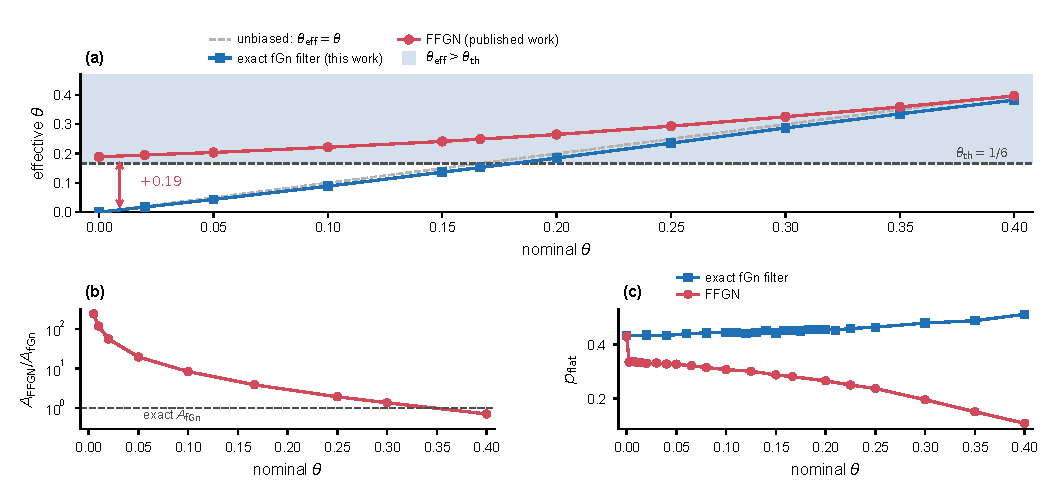
\includegraphics[width=\textwidth]{fig1_generator}
  \caption{\label{fig:gen} The FFGN construction examined here
  does not connect continuously to uncorrelated noise. (a) Shape-matched
  effective exponent $\theff$ measured on the \emph{binarised} field against the
  nominal $\theta$ of each generator; the FFGN family (circles) is offset
  upwards by $+0.19$ at $\theta_{\mathrm{nom}}=0$ and lies entirely inside the shaded
  region $\theff>\thth$, so no member with $\theta_{\mathrm{nom}}\ge0$ reaches the
  short-range KPZ regime, whereas the exact fractional-Gaussian-noise filter
  (squares) is unbiased and passes through the origin. (b) Fitted correlation
  amplitude ratio $A_{\mathrm{FFGN}}/A_{\mathrm{fGn}}$: $A_{\mathrm{FFGN}}$ stays of order
  unity for all $\theta$ while the exact amplitude $2\theta(\theta+\frac12)$
  vanishes, so the ratio diverges as $\theta\to0$ and
  crosses unity only near $\theta\approx0.35$ (the point at $\theta=0$ is
  omitted because the exact amplitude is exactly zero there). (c) Consequence
  inside the model itself at
  $L=256$: the structural order parameter $p_{\mathrm{flat}}$ jumps by $23\%$ between
  true white noise and $\mathrm{FFGN}(\theta\to0)$ and then \emph{decreases} with
  $\theta$, while the corrected generator gives a continuous, monotonically
  increasing dependence. All three panels span the same range
  $\theta_{\mathrm{nom}}\in[0,0.40]$.}
\end{figure*}

\begin{figure*}[t]
  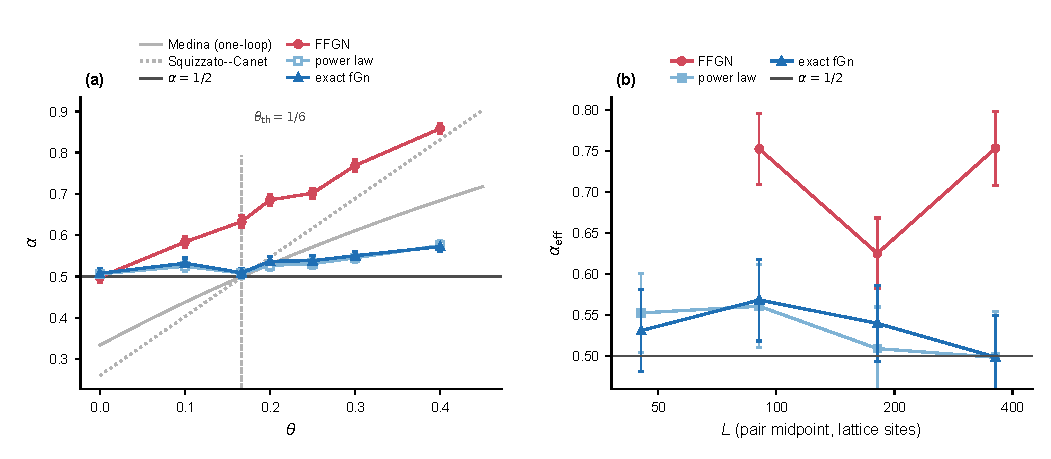
\includegraphics[width=\textwidth]{fig2_exponents}
  \caption{\label{fig:exp} The measured roughness exponent is
  generator-dominated. (a) $\alpha$ from $W_{\mathrm{sat}}\sim L^{\alpha}$ with
  bootstrap errors obtained by resampling runs, for three generators, against
  the Medina one-loop and Squizzato--Canet long-range branches. The two
  corrected filters (open squares: power-law filter; filled triangles: exact
  fractional-Gaussian-noise filter) agree to within $0.008$ everywhere, while
  FFGN lies $0.16$--$0.29$ higher and reaches $0.86$ at $\theta=0.4$. (b)
  $\alpha_{\mathrm{eff}}$ from consecutive size pairs at $\theta=0.25$, with
  bootstrap errors, against the pair midpoint $L$: both corrected filters drift
  \emph{down} towards $1/2$ as $L$ grows, whereas the FFGN value does not.}
\end{figure*}

\begin{figure*}[t]
  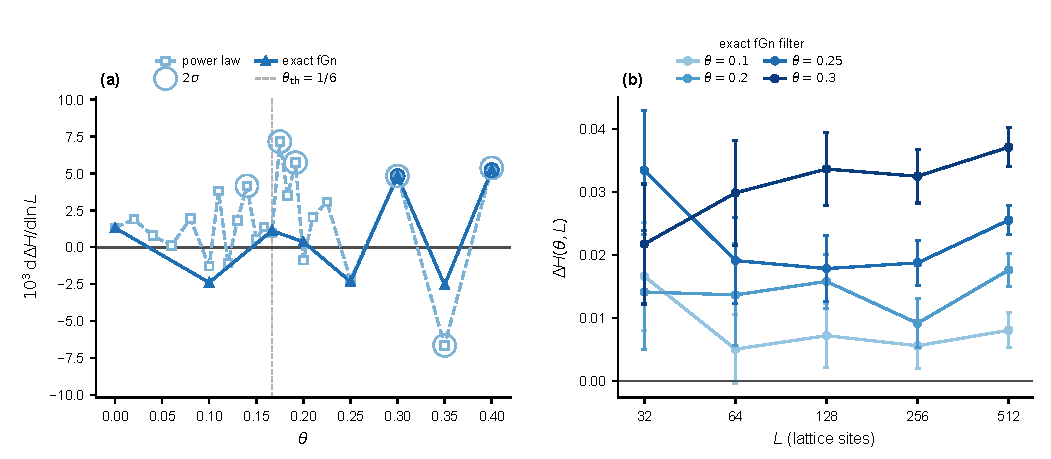
\includegraphics[width=\textwidth]{fig3_fixed_theta}
  \caption{\label{fig:fixed} The decisive test: at \emph{fixed} $\theta$ a
  genuine crossover requires the deviation from the KPZ reference to grow with
  $L$. (a) $\mathrm{d}\,\Delta H/\mathrm{d}\ln L$, the slope of the deviation
  against $\ln L$, in units of $10^{-3}$, for the two corrected filters; open
  rings mark points whose slope is significant at the $2\sigma$ level (outer
  ring: power-law filter, inner ring: exact fractional-Gaussian-noise filter).
  Below $\theta=0.25$ the slopes scatter about zero and are individually
  insignificant. Positive slopes become systematic only for
  $\theta\ge0.30$; individual two-sigma rings are not interpreted on their own,
  because no correction for multiple comparisons is applied
  (Appendix~\ref{app:stats}).
  (b) The underlying deviation $\Delta H(\theta,L)$ versus $L$
  for the exact fractional-Gaussian-noise filter at four values of $\theta$.
  The series at $\theta=0.10$, $0.20$ and $0.25$ show no trend within their
  bootstrap errors, while the $\theta=0.30$ series rises monotonically from
  $0.022$ at $L=32$ to $0.037$ at $L=512$. Within this window, therefore, no
  crossover is resolved at the smaller values; where it lies beyond the window
  is left open by these data.}
\end{figure*}

\begin{figure*}[t]
  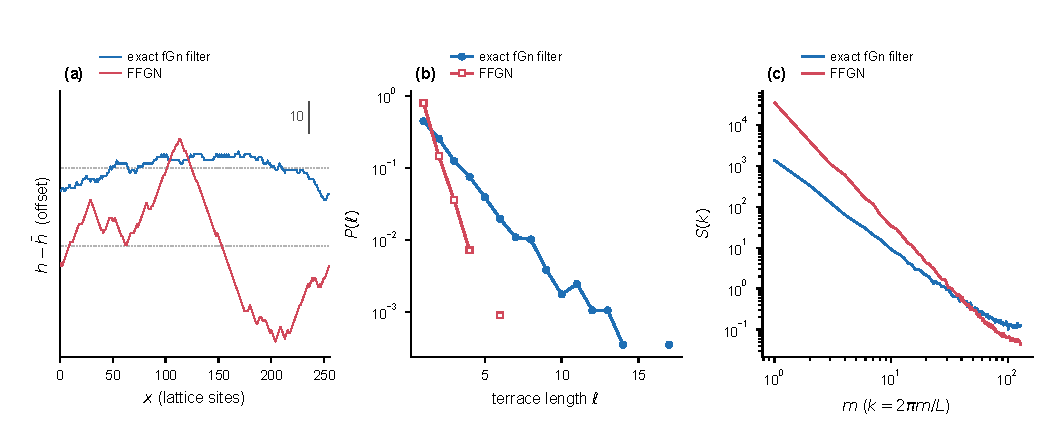
\includegraphics[width=\textwidth]{fig4_morphology}
  \caption{\label{fig:morph} The interface morphology inverts between the two
  generators at $L=256$ and $\theta=0.40$. (a) Representative profiles (single
  realisation, successive profiles offset vertically and separated by dotted
  baselines; the bar denotes ten height units). The corrected generator keeps
  the KPZ-like alternation of short terraces and unit steps, whereas the FFGN
  surface develops very large excursions. (b) Flat-terrace length distribution
  $P(\ell)$; the mean terrace length rises from $1.88$ to $2.24$ lattice units
  between $\theta=0$ and $0.40$ under the corrected generator but
  \emph{falls} to $1.25$ under FFGN. Empty bins are omitted rather than
  floored. (c) Structure factor $S(k)$; the FFGN spectrum develops a markedly
  steeper large-$k$ slope, the signature in which the reported faceting and
  anomalous scaling are diagnosed \cite{AlesLopez2019,SongXia2021PRE}.}
\end{figure*}

\subsection{Validation and characterisation of the two generators}
\label{sec:gen}

\textbf{The model reproduces KPZ at $\theta=0$.} For the FFGN-driven BD model
with $L=128\dots1024$ and $T=2\times10^{5}$ sweeps, a fit of
$W_{\mathrm{sat}}\sim L^{\alpha}$ gives $\alpha=0.4964$, $W_{\mathrm{sat}}/\sqrt L$
is constant to within $10\%$ over that range, and the growth exponent approaches
$\beta=1/3$ in the growth window. The saturation time obeys
$t_\times\simeq0.6\,L^{3/2}$ sweeps, with no large prefactor, which sets the
simulation length used throughout. Over a common window $L=64,128,256$ the same
fit gives $\alpha=0.5019$ (FFGN) and $\alpha=0.5088$ (spectral).

\textbf{The FFGN implements the imposed exponent but not the imposed amplitude.}
The temporal correlation function of the FFGN sequence reproduces the target
slope $2\theta-1$ well for all $\theta$: over $\tau\in[64,4096]$ we measure
$-0.907$ against $-0.900$ expected at $\theta=0.05$, and $-0.659$ against
$-0.667$ at $\theta=1/6$; the binarised noise has $P(\ders=1)=0.4996$--$0.5020$
in every case. The amplitude, however, is wrong at small $\theta$. Fitting
$|C_\eta(\tau)|=A\tau^{2\theta-1}$ over the same window gives
$A_{\mathrm{FFGN}}$ between $1.27$ and $0.42$ across
$\theta\in[0,0.45]$, i.e.\ essentially $\theta$-independent, whereas the exact
fractional-Gaussian-noise correlator carries the amplitude
$A_{\mathrm{fGn}}=2\theta(\theta+\tfrac12)$ and vanishes as $\theta\to0$. The
ratio $A_{\mathrm{FFGN}}/A_{\mathrm{fGn}}$ is $245$ at $\theta=0.005$, $120$ at
$0.01$, $20$ at $0.05$, $8.4$ at $0.10$, $3.9$ at $1/6$, $1.9$ at $0.25$ and
$0.7$ at $0.40$. Directly, the binarised FFGN sequence at
$\theta_{\mathrm{nom}}=10^{-9}$ has $C(1)/C(0)=0.195$ and a
$C(\tau)\propto\tau^{-1}$ tail, whereas white noise has $C(\tau)=0$ for
$\tau\ge1$.

\textbf{The effect is intrinsic, not a truncation artefact.} The FFGN represents
$C(\tau)$ as a sum of $N$ AR(1) components on a geometric grid of inverse time
scales. Increasing $N$ extends the grid towards slower modes, so a truncation
artefact would disappear as $N$ grows. It does not: at $\theta=0$ the fitted
amplitude is $1.3558$, $1.3559$ and $1.3559$ for $N=23$, $32$ and $48$, i.e.\
fully converged. Equation~\eqref{eq:affgn} shows why: the geometric $u$-grid
makes $\sum_n W_n^2e^{-u_n\tau}/(1-r_n^2)$ tend to a constant times
$\tau^{-1}$, and the factor $2\theta(\theta+\tfrac12)$ that should suppress that
tail is simply absent from the standard weights.

\textbf{Binarised calibration.} Because the model uses $\ders=\mathbf 1[\eta>0]$
and thresholding compresses correlations through
$C_{\mathrm{bin}}=(2/\pi)\arcsin C$, the calibration must be performed on the
binarised field. Matching $C_{\mathrm{bin}}(\tau)$ to the binarised exact
fractional-Gaussian-noise family over $\tau\in[1,4096]$ by weighted least squares
gives the effective $\theta$ reported in Fig.~\ref{fig:gen}(a).

We use $\theff$ strictly as a \emph{shape-matched diagnostic for the binarised
correlation function}. It is a single fitted number summarising the whole
correlation curve, and it must not be read as an exact reparameterisation of the
FFGN construction, of the dynamical renormalisation-group coupling, or of the
universality class. Three distinct quantities appear in this paper and are kept
separate throughout: (i) the \emph{nominal} $\theta$ of a generator, which is the
parameter the published work varies; (ii) the \emph{shape-matched} $\theff$,
which is the diagnostic just defined; and (iii) the
\emph{temporal-correlation exponent} of the continuum theory entering
Eqs.~\eqref{eq:noise} and~\eqref{eq:thetath}. Two generators with the same
$\theff$ need not have the same correlation function at intermediate lags or the
same low-frequency weight, and Sec.~\ref{sec:artefact} exhibits exactly that
residual difference. Accordingly, statements below of the form
``$\theff>\thth$'' mean only that the fitted binarised correlation curve lies in
the range where the theory predicts long-range behaviour; they do not identify
$\theff$ with the exponent of that theory.

The results are decisive:
\begin{itemize}
\item the FFGN family gives $\theff=0.1888$ at $\theta_{\mathrm{nom}}=0$, i.e.\
\emph{above} the renormalisation-group threshold $\thth=1/6$, and
$\theff\ge0.1888$ for every $\theta_{\mathrm{nom}}\ge0$; the offset is
approximately $\theff\simeq0.19+0.44\,\theta_{\mathrm{nom}}$;
\item the spectral family gives $\theff=0.0000$ at $\theta_{\mathrm{nom}}=0$ ---
exactly white noise --- and $\theff\simeq0.95\,\theta_{\mathrm{nom}}$
thereafter, i.e.\ it is an essentially unbiased realisation of the intended
$\theta$ axis.
\end{itemize}
The FFGN family therefore never samples the short-range KPZ regime
$\theff<\thth$ for any non-negative nominal $\theta$.

\subsection{The generator bias in the full model}
\label{sec:artefact}

The bias is not a property of the noise alone; it changes the interface.
Because the model is single-step, the structural order parameter is
$p_{\mathrm{flat}}=\mathrm{frac}\{\Delta h=0\}$ of Eq.~\eqref{eq:pflat}. At
$L=256$ with $128$ realisations we find
\begin{center}
\compacttab
\begin{tabular}{lccc}
\hline
noise & $\theta$ & $p_{\mathrm{flat}}$ & $W_{\mathrm{sat}}$\\
\hline
i.i.d.\ (true white)      & $0$        & $0.4366$ & $3.62$\\
FFGN                      & $10^{-9}$  & $0.3359$ & $5.61$\\
FFGN                      & $0.05$     & $0.3243$ & $6.20$\\
spectral                  & $0$        & $0.4321$ & ---\\
spectral                  & $0.05$     & $0.4369$ & ---\\
spectral                  & $1/6$      & $0.4504$ & ---\\
spectral                  & $0.25$     & $0.4635$ & ---\\
\hline
\end{tabular}
\end{center}
The FFGN produces a $23\%$ \emph{discontinuity} of $p_{\mathrm{flat}}$ between
true white noise and its own $\theta\to0$ limit, and its $p_{\mathrm{flat}}$
then \emph{decreases} with $\theta$. The spectral family is continuous and
increases monotonically, from $0.4321$ at $\theta=0$ to $0.5177$ at
$\theta=0.40$ (Fig.~\ref{fig:gen}(c)). A generator that inverts the sign of
the $\theta$-dependence of the model's order parameter cannot be used to locate
a threshold in that parameter.

The same contrast appears in the measured exponents. Over the common window
$L=64,128,256$, $\alpha$ rises from $0.5019$ to $0.8419$ between
$\theta_{\mathrm{nom}}=0$ and $0.40$ when the FFGN generator is used, but only
from $0.5088$ to $0.5638$ with the $\theta$-continuous generator
(Fig.~\ref{fig:exp}(a)). The measured $\theta$-dependence of $\alpha$ in this
model is thus dominated by the noise generator rather than by an intrinsic
change of universality class. Consistently, the iForest diagnostic, whose
features are exactly the roughness-scaling quantities from which $\alpha$ is
built, barely responds in the corrected track ($|z|<2$ for all $\theta\le0.4$),
while the distributional diagnostic responds strongly ($z$ up to $30$): over the
accessible range the change in the interface is a local, one-parameter effect
rather than a restructuring of the multi-scale roughness geometry.

\subsection{Negative-$\theta$ control}
\label{sec:res:neg}

The spectral family permits $\theta<0$, which no previous study of this model
has simulated. There the long-range coupling has canonical dimension
$[w_\theta]=4\theta<0$ and is irrelevant, so uncorrelated-noise exponents
should be restored. We find exactly that: over $L=32\dots256$ the fitted
roughness exponent is $\alpha=0.4947\pm0.0181$, $0.5028\pm0.0070$,
$0.4993\pm0.0092$ at $\theta=-0.2,-0.1,-0.05$, all consistent with $1/2$, while
$p_{\mathrm{flat}}$ does drop below its $\theta=0$ value
($0.4205$ against $0.4333$ at $L=256$). The control therefore separates two
things that the diagnostics could otherwise conflate: the noise is measurably
different, but the universality class is not.

\subsection{Why the onset-drift method cannot locate $\thc$ here}
\label{sec:res:diag}

\textbf{In nominal FFGN units both diagnostics return $\thc=0$.} Analysing the
FFGN track ($L=64\dots512$, 22 values of $\theta$, up to 256 realisations per
cell) gives, for the distributional diagnostic, $\thc=0.0002\pm0.0007$ with
$\chi^2/\mathrm{dof}=0.17/1$, and for the Isolation Forest,
$\thc=0.0001\pm0.0011$; the onset is pinned at the smallest non-zero $\theta$
available on the grid for every $L$. This is the expected signature of
Sec.~\ref{sec:artefact}: since $\mathrm{FFGN}(\theta_{\mathrm{nom}}=0)$ already
carries $\theff=0.19>\thth$, shape-based observables see a long-range interface
as soon as the noise differs from $\theta=0$ at all. It is a direct explanation
of the published claim that the KPZ phase is destroyed for any $\theta>0$.
Because the reference ensemble at $\theta=0$ is true white noise while every
$\theta>0$ cell uses FFGN, this particular onset measures the generator
discontinuity itself and is not a measurement of $\thc$.

\textbf{On the corrected axis the same analysis appears to give a clean drift
--- and that drift is an artefact.} For these comparisons every
$(\theta,L)$ cell of both corrected-generator campaigns was reduced to a
\emph{common} $96$ realisations before either diagnostic was evaluated, so that
statistical power is identical across every size and every $\theta$; this is a
subsample of the $192$ realisations stored per cell at $L\le256$, and equals the
full stored count at $L=512$ (Table~\ref{tab:runs}). The fixed-significance
onset of the distributional diagnostic
decreases monotonically over a factor of $16$ in $L$,
\begin{center}
\compacttab
\begin{tabular}{lccccc}
\hline
 & \multicolumn{5}{c}{$\theta^*(L)$}\\
\cline{2-6}
$L$ & 32 & 64 & 128 & 256 & 512\\
\hline
$z\ge3$ & $0.2415$ & $0.2336$ & $0.1710$ & $0.1375$ & $0.0823$\\
$z\ge5$ & $0.3306$ & $0.3073$ & $0.2686$ & $0.2410$ & $0.1471$\\
\hline
\end{tabular}
\end{center}
with a forced-zero finite-size-scaling collapse that is formally excellent
($A=0.92$, $1/\nu=0.36$, $\chi^2/\mathrm{dof}=0.75/3$, $p=0.86$ for $z\ge3$),
and at $L=512$ the onset lies well below $1/6$. Read alone, this would exclude a
threshold at $1/6$. It does not, and the reason is the key methodological point
of this paper.

The split-half null floor of the distributional diagnostic is not a constant: it
decreases with system size, from $0.0109$ at $L=32$ to $0.0024$ at $L=512$
(a factor of $4.5$), because a larger $L$ gives more columns per
realisation and hence a less noisy per-run pmf. A criterion of the form
``$\Delta H$ exceeds $z$ null standard deviations'' therefore necessarily
crosses at a smaller $\theta$ as $L$ grows \emph{even if the physics is
completely scale-free}. Matching the number of runs --- which we did, and which
is necessary --- does not remove this, because the $L$-dependence enters through
the number of \emph{columns}, not the number of runs.

\textbf{The decisive test is at fixed $\theta$.} If the model possesses a
crossover length $\xi_\times(\theta)$ that grows as $\theta\to0^{+}$, then for a
fixed $\theta$ the surface is KPZ-like at scales below $\xi_\times$ and
long-range above it, so increasing $L$ resolves \emph{more} of the long-range
behaviour and the deviation from the $\theta=0$ reference must \emph{grow} with
$L$. If instead the deviation is a purely local, one-point effect, it is
$L$-independent. Figure~\ref{fig:fixed}(b) shows the outcome: over
$L=32\dots512$, $\Delta H(\theta,L)$ at fixed $\theta$ is \emph{$L$-independent}
within errors for every $\theta$ from $-0.2$ to $0.4$; the fitted slopes
$\mathrm{d}\,\Delta H/\mathrm{d}\ln L$ of Fig.~\ref{fig:fixed}(a) are
statistically indistinguishable from
zero for all but four of the 26 values of $\theta$, with no systematic sign. The
deviation is therefore a smooth local parameter, not a crossover signature, and
the apparent onset drift of the previous paragraph tracks the shrinking null
floor rather than any change of scaling behaviour. We report this explicitly
because the same construction underlies the Hellinger-distance threshold of
Ref.~\cite{WangXia2025}: a fixed-significance crossing of a distributional
distance cannot be used to locate a crossover unless the fixed-$\theta$
scale-dependence of that distance has first been shown to be non-trivial.

\textbf{The exponent evidence, with honest error bars.} The same conclusion
follows, independently, from the roughness exponent, provided the errors are
computed by resampling runs rather than from the residuals of a fit to four or
five points. The latter procedure understates the uncertainty by almost an order
of magnitude in our data (it gives $\pm0.0016$ where a run bootstrap gives
$\pm0.0127$). With bootstrap errors, over $L=32\dots512$ (the bootstrap uncertainty on
every entry below is $\pm0.011$--$0.015$, i.e.\ it is the last digit or two and
is omitted from the table for width):
\begin{center}
\compacttab
\begin{tabular}{lccccc}
\hline
$\theta$ & $-0.2$ & $0$ & $1/6$ & $0.25$ & $0.40$\\
\hline
FFGN       & ---      & $0.4986$ & $0.6330$ & $0.7019$ & $0.8585$\\
corrected  & $0.4947$ & $0.5062$ & $0.5082$ & $0.5311$ & $0.5750$\\
\hline
\end{tabular}
\end{center}
With the corrected generator the exponent is consistent with $1/2$ everywhere up
to $\theta=1/6$, marginally above it at $\theta=0.25$ ($2.6\sigma$, $\alpha=0.5311\pm0.0120$)
and clearly above it only at $\theta=0.4$ ($\alpha=0.575$). The FFGN generator
gives $\alpha=0.63$ and $0.70$ at the same nominal $\theta=1/6$ and $0.25$,
i.e.\ the published deviations are an order of magnitude larger than those of
the corrected model at the same nominal parameter.

Moreover, $\alpha_{\mathrm{eff}}$ extracted from consecutive size pairs
(Fig.~\ref{fig:exp}(b)) \emph{decreases} towards $1/2$ as $L$ grows for the
spectral generator at $\theta\ge1/6$ --- for $\theta=0.20$ the sequence is
$0.598,0.533,0.497,0.491$ over $L$ pairs $32\!\to\!64,\dots,256\!\to\!512$, and
for $\theta=0.25$ it is $0.553,0.561,0.509,0.498$ --- whereas for the FFGN at
the same nominal $\theta$ it does not decrease ($\theta=0.25$:
$0.753,0.625,0.754$; $\theta=0.4$: $0.815,0.868,0.888$). The corrected
deviations behave like finite-size corrections that vanish as $L$ grows; the
FFGN deviations behave like asymptotic behaviour. This is the sharpest form of
our central result: at the accessible scales the $\theta$-dependence reported in
the literature is a property of the noise generator, and with a
$\theta$-continuous generator the crossover to the long-range branch lies beyond
$L\approx512$ for $\theta\le0.25$.

\textbf{Diagnostic performance, honestly reported.} Three candidate
distributional observables were rejected with data rather than assumed away.
With matched run counts the split-half null floor of the Hellinger distance is
$0.0024$--$0.0109$ for the exact increment pmf and $0.024$--$0.099$ for the
exact terrace-length pmf, against $0.080$--$0.181$ for a histogrammed
standardised height-difference density and $0.102$--$0.251$ for a histogrammed
standardised height density. The latter two are therefore not merely noisy:
their floor exceeds the physical signal over the entire range, and the height
density is insensitive by construction at the $1\%$ level ($\Delta H$ consistent
with zero, $|z|<2.7$, in every cell of both tracks). Because the increment pmf
carries only $p_{\mathrm{flat}}$ (Sec.~\ref{sec:model:singlestep}), and because
the $L$-independence of $\Delta H$ shows that $p_{\mathrm{flat}}$ is a local
parameter with no scale dependence, this diagnostic is in the end a calibrated
probe of a single non-universal quantity. It detects the generator bias
unambiguously; it cannot, on its own, locate a crossover.


% =====================================================================
\subsection{Exponents and morphology: the same conclusion}
\label{sec:res:morph}

Table~\ref{tab:morph} contrasts the two generators at $L=256$ over a range of
nominal $\theta$. At $\theta=0$ the two tracks agree to within their statistical
errors in every quantity, as they must, since there the reference is the same
white noise. They diverge dramatically as $\theta$ grows.

\begin{table}[htbp]
\centering
\caption{\label{tab:morph} Exponents and morphology at $L=256$ for the FFGN
(published) and spectral ($\theta$-continuous) generators at matched nominal
$\theta$. $\alpha_s$ is the spectral roughness exponent, $p_{\mathrm{flat}}$ the
flat-pair fraction and $W_{\mathrm{sat}}$ the saturated width. For each quantity the
left column is the FFGN (published) generator and the right column the
$\theta$-continuous exact-fGn filter.}
\compacttab
\begin{tabular}{lcccccc}
\hline
$\theta$ & \multicolumn{2}{c}{$\alpha_s$} & \multicolumn{2}{c}{$p_{\mathrm{flat}}$}
         & \multicolumn{2}{c}{$W_{\mathrm{sat}}$}\\
\cline{2-3}\cline{4-5}\cline{6-7}
 & FFGN & fGn & FFGN & fGn & FFGN & fGn\\
\hline
$0$    & $0.514$ & $0.516$ & $0.433$ & $0.434$ & $3.65$ & $3.62$\\
$0.10$ & $0.694$ & $0.529$ & $0.308$ & $0.444$ & $6.81$ & $3.65$\\
$1/6$  & $0.753$ & $0.536$ & $0.281$ & $0.451$ & $8.06$ & $3.81$\\
$0.20$ & $0.774$ & $0.512$ & $0.267$ & $0.457$ & $8.84$ & $3.88$\\
$0.25$ & $0.821$ & $0.568$ & $0.236$ & $0.465$ & $10.20$ & $3.92$\\
$0.40$ & $1.049$ & $0.548$ & $0.111$ & $0.511$ & $17.99$ & $4.05$\\
\hline
\end{tabular}
\end{table}

Three features stand out. First, the \emph{sign} of the morphological response
is opposite in the two tracks: under FFGN the flat-pair fraction
\emph{collapses}, from $0.433$ to $0.111$ at $\theta=0.4$, so the interface
becomes almost entirely stepped and the mean terrace length shrinks from $1.90$
to $1.24$ lattice units, whereas under the corrected generator the flat-pair
fraction \emph{rises} to $0.511$ and terraces \emph{lengthen} to $2.23$ units.
Because the model is single-step (Sec.~\ref{sec:model:singlestep}) the only
morphology available is terraces and unit steps, and the two generators drive
that single degree of freedom in opposite directions. Second, the spectral
roughness exponent --- the quantity in which the reported faceting and anomalous
scaling are diagnosed \cite{AlesLopez2019,SongXia2021PRE} --- saturates at
$0.52$--$0.57$ under the corrected generator but climbs to $1.05$ under FFGN at
$\theta=0.4$, reproducing the published trend towards faceted, super-rough
surfaces. Third, the saturated width is inflated by a factor of $4.4$ at
$\theta=0.4$ ($17.99$ against $4.05$), which is exactly the amplitude effect
that any un-normalised observable would mistake for a transition
(Sec.~\ref{sec:diag}). The growth exponent behaves consistently: it is flat at
$\beta=0.23$--$0.30$ for the corrected generator across the whole range but
rises from $0.267$ to $0.470$ under FFGN.

Each morphological and dynamical signature that has been used to argue for a
long-range phase in this model --- faceting diagnosed from the spectral
exponent, terrace hardening, an inflated saturated width, and a rising growth
exponent --- is present in the FFGN track, and absent or an order of magnitude
weaker in the corrected one, over the range of $\theta$ and $L$ we can access.
Figure~\ref{fig:morph} shows the two tracks side by side at $\theta=0.40$: the
corrected surface keeps the KPZ-like alternation of short terraces and unit
steps, whereas the FFGN surface is dominated by very large excursions, its
terrace-length distribution hardens, and its structure factor acquires a
markedly steeper large-$k$ slope --- the very signature in which the reported
faceting and anomalous scaling are diagnosed
\cite{AlesLopez2019,SongXia2021PRE}.

\subsection{Supplementary check with the exact fractional-Gaussian-noise
filter}
\label{sec:res:fgn}

The conclusion of Secs.~\ref{sec:res:diag}--\ref{sec:res:morph} rests on a
spectral family that under-correlates relative to exact fractional Gaussian
noise at large $\theta$, which is the one systematic that could in principle
reconcile our exponents with the long-range branches. We therefore repeated the
measurement with the exact-spectrum filter of Eq.~\eqref{eq:fgnspec}, over
$\theta=0,\,0.10,\,1/6,\,0.20,\,0.25,\,0.30,\,0.35,\,0.40$ and
$L=32\dots512$, with the same protocol, the same number of realisations and the
same diagnostics.

\textbf{Roughness exponent.} With bootstrap errors over independent
realisations,
\begin{center}
\compacttab
\begin{tabular}{lccc}
\hline
$\theta$ & FFGN & power-law & exact fGn\\
\hline
$0$    & $0.4986$ & $0.5062$ & $0.5076$\\
$1/6$  & $0.6330$ & $0.5082$ & $0.5089$\\
$0.20$ & $0.6855$ & $0.5269$ & $0.5368$\\
$0.25$ & $0.7019$ & $0.5311$ & $0.5383$\\
$0.40$ & $0.8585$ & $0.5750$ & $0.5724$\\
\hline
\end{tabular}
\end{center}
The two corrected filters agree with each other to within $0.008$ at every
$\theta$ --- well inside their errors --- whereas the FFGN values lie $0.16$
($\theta=0.25$) to $0.29$ ($\theta=0.40$) higher. The amplitude deficit of the
power-law filter is therefore quantitatively negligible for the conclusion, and
the gap to the published exponents survives the exact filter by a factor of
twenty. All three tracks give $\beta=0.25$--$0.26$, flat in $\theta$.

\textbf{Fixed-$\theta$ scaling test.} The decisive test of
Sec.~\ref{sec:res:diag} repeated with the exact filter gives, for the slope
$\mathrm{d}\,\Delta H/\mathrm{d}\ln L$:
\begin{center}
\compacttab
\begin{tabular}{lcc}
\hline
$\theta$ & slope & sig.?\\
\hline
$0.10$ & $-0.0024$ & no\\
$1/6$  & $+0.0011$ & no\\
$0.20$ & $+0.0004$ & no\\
$0.25$ & $-0.0023$ & no\\
$0.30$ & $+0.0048$ & \textbf{yes}\\
\hline
\end{tabular}
\end{center}
At $\theta=0.20$ and $0.25$ the deviation remains $L$-independent, confirming
that the crossover is not resolved at these values within $L\le512$, and
reproducing the power-law result. At $\theta\ge0.30$, however, the dependence
becomes systematically \emph{positive} ($+0.0048$ at $0.30$ and $+0.0052$ at
$0.40$, both well outside the errors), which is the signature of the crossover
entering the accessible window: the deviation now grows with $L$, as a genuine
crossover requires.

\textbf{Effective exponent from size pairs.} At $\theta=0.20$ the exact filter
gives $\alpha_{\mathrm{eff}}=0.552,\,0.572,\,0.506,\,0.516$ over the size pairs
$32\!\to\!64,\dots,256\!\to\!512$, and at $\theta=0.25$ it gives
$0.531,\,0.568,\,0.540,\,0.499$; both decline towards $1/2$, as the power-law
filter does, while the FFGN values at the same nominal $\theta$ show no decline
($0.694,0.694,0.666$ and $0.753,0.625,0.753$). The exact filter therefore
reproduces every qualitative feature of Sec.~\ref{sec:res:diag} and shifts the
numbers by less than their error bars.

Taken together, the supplementary campaign closes the main systematic of this
work. The corrected roughness exponent remains within $0.08$ of $1/2$ for
$\theta\le0.4$, the deviation is $L$-independent for $\theta\le0.25$ at
$L\le512$ and becomes $L$-dependent only for $\theta\ge0.30$, and none of this
resembles the published behaviour, which we reproduce only when the FFGN
generator is used.

\section{Discussion}
\label{sec:discussion}
% =====================================================================

\subsection{Why the nominal $\theta$ axis is not the physical one}

The model family is specified by the correlator
$\langle\eta\eta\rangle\propto|t-t'|^{2\theta-1}$ or, equivalently, by
Eq.~\eqref{eq:noise}. Both statements degenerate at $\theta=0$: the power law
becomes $\tau^{-1}$, which is emphatically \emph{not} white noise. Whiteness at
$\theta=0$ is an additional requirement that any generator must impose
separately, and the physically correct way to impose it is to carry the exact
fractional-Gaussian-noise amplitude $2\theta(\theta+\tfrac12)$, which vanishes
at the origin. Mandelbrot's FFGN does not do this: its weights depend on
$\theta$ only through the power $u_n^{1-2\theta}$ and the prefactor
$B^{1/2-\theta}-B^{\theta-1/2}$, neither of which vanishes as $\theta\to0$ in
the required way. The consequence is a correlation floor of order
$C(1)/C(0)\simeq0.19$ that is present at \emph{every} nominal $\theta$ we
simulated, including $\theta=0$. For the parameter values that we could verify
first-hand (Table~\ref{tab:lit}), the same construction is used, so the floor
should be present there as well; where the published description does not
specify the generator, we make no claim.

This single fact organises several otherwise puzzling published results. It
predicts that FFGN-based simulations should see long-range behaviour at any
$\theta>0$ \cite{SongXia2016,SongXia2021PRE,SongXia2021JSTAT,RodriguezFernandez2024},
that the threshold inferred from macroscopic dynamics should differ from the one
inferred from fluctuation statistics \cite{JiangXia2026}, and that the measured
exponents should vary with $\theta$ far more strongly than the underlying model
requires. All three are observed in the sources listed in Table~\ref{tab:lit}.

\subsection{The bias does not simply rescale $\thc$}

It is tempting to conclude that the published $\thc=0.25$ ``really means''
$\thth=1/6$ once the $\theta$ axis is recalibrated. Our calibration says
otherwise. The binarised mapping takes
$\theta_{\mathrm{nom}}=0.25$ to $\theff=0.2934$, i.e.\ \emph{further} from
$1/6$, not closer, and the same holds at $1/6$ ($\theff=0.2492$). We therefore
do not reinterpret the literature; we report a measurement made on a
$\theta$ axis that is continuous at the origin.

A residual generator dependence survives even after matching $\theff$. At
$\theff\simeq0.25$ the FFGN gives $\alpha\simeq0.62$ and the spectral family
$\alpha\simeq0.56$; at $\theff\simeq0.39$, $0.86$ against $0.55$. A single
effective exponent is not a complete characterisation of the noise: the FFGN
correlation function is not of the exact fractional-Gaussian form at
intermediate lags, and its surplus low-frequency weight is not captured by a
one-parameter shape match. This is a limitation of our calibration, and it means
that the corrected-track exponents should be attributed to the spectral family
specifically, not to ``the'' continuum model.

\subsection{What the corrected measurement does and does not establish}

With a $\theta$-continuous generator the roughness exponent is consistent with
$1/2$ for all $\theta\le1/6$, marginally above it at $\theta=0.25$ and equal to
$0.575\pm0.012$ at $\theta=0.4$, while the growth exponent is flat at
$0.24$--$0.28$. Extracted from consecutive size pairs, $\alpha_{\mathrm{eff}}$
decreases towards $1/2$ as $L$ grows for $\theta\ge1/6$, and at fixed $\theta$
the deviation of the increment density from the KPZ reference does not grow with
$L$. We therefore \emph{cannot} report a measured $\thc$: on the accessible
scales the crossover to the long-range branch has not been reached for
$\theta\le0.25$, so no onset exists to locate, and the apparent onset produced by
the standard method is a property of the detection floor.

This is a negative result for the methodology rather than for the theory. It is
consistent with the renormalisation-group prediction $\thth=1/6$: within the
window we can access, the prediction is not contradicted by anything we measure.
It is not confirmed either, because $\theta>1/6$ would then be expected to show a
long-range regime already at $L\approx512$, and it does not clearly do so. What
the data do establish is that the deviations
reported at $\theta\simeq0.2$--$0.25$ are an order of magnitude larger under
FFGN than under a generator with the correct correlation amplitude at the same
nominal $\theta$, and that they behave asymptotically under FFGN while shrinking
with $L$ under the corrected generator.

Two caveats must be stated plainly. (i) The power-law filter of
Eq.~\eqref{eq:spectral} is cut off at the Nyquist frequency, so it
under-correlates relative to exact fractional Gaussian noise at large $\theta$
and its binarised $\theta$ axis is accurate only to about $10\%$. Because a
weaker long-range coupling implies a larger crossover length, this was the one
systematic that could have produced a spuriously flat $\alpha$; it is discharged
by the independent campaign of Sec.~\ref{sec:res:fgn}, which used a filter
carrying the exact fractional-Gaussian-noise spectral density and hence a
$\theta$ axis accurate to $1\%$. That campaign reproduces every qualitative
feature we checked against the power-law results and moves $\alpha$ by at most
$0.008$, an order
of magnitude less than the $0.16$--$0.29$ gap to the FFGN values and far less
than the gap to the long-range branches. (ii) The accessible dynamic range is
$L=32\dots512$. The fixed-$\theta$ test detects the crossover only for
$\theta\ge0.30$, so there is no measured $\thc$. The decisive experiment is
therefore a larger one, and we state the target as an extrapolation from our
present trend rather than as a prediction: on the observed growth of
$\mathrm{d}\,\Delta H/\mathrm{d}\ln L$ with $\theta$, sizes of order
$L\gtrsim4096$ at matched realisation count would be needed for the
$\theta\le0.25$ crossover to enter the window, at which point the long-range
exponents themselves become measurable. We have not performed that campaign and
cannot claim that the crossover behaves as this extrapolation assumes.

\subsection{Methodological lessons for this class of study}
\label{sec:disc:lessons}

Five failure modes, each of which we encountered and measured, are worth
recording because they are easy to fall into and hard to notice. We state them
in order of how much damage they did.

\emph{A generator must be validated by plotting $C(\tau)/C(0)$ against the exact
fractional-Gaussian form, and must be required to reproduce white noise at
$\theta=0$.} Reproducing the correct power-law exponent is not sufficient: the
FFGN does so while being wrong by a factor of $245$ in amplitude at
$\theta=0.005$.

\emph{Any observable that retains the fluctuation amplitude will report a
transition at $\theta=0^+$.} For any $\theta>0$ the noise spectral density
diverges at low frequency, so the saturated width grows with $\theta$ even when
the universality class does not. This is what made our first Isolation-Forest
implementation fire at the smallest non-zero $\theta$ on the grid.

\emph{Histogramming a discrete distribution before computing a Hellinger
distance is invalid.} Standardising the samples moves the support, the spikes of
the two ensembles land in disjoint bins, and $H$ saturates near its maximum. The
exact pmf must be used; the difference in null floor is a factor of $20$--$30$.

\emph{Statistical power must be matched across system sizes --- and even then a
fixed-significance onset is not interpretable.} An unmatched ensemble size made
an Isolation-Forest onset drift from $0.215$ to $0.002$ with no physical cause,
and a campaign with half the realisations at $L=512$ produced a non-monotonic
onset sequence that appeared to signal saturation; matching run counts removed
both artefacts. Matching is nonetheless \emph{not} sufficient: the split-half
floor also falls with $L$, because a larger $L$ gives more columns per
realisation, so a fixed-significance crossing keeps drifting towards smaller
$\theta$ even when the observable is entirely $L$-independent. The remedy is to
test the observable's scale dependence at \emph{fixed} $\theta$ before any onset
is extracted, and to prefer effect-size over significance criteria.

\emph{Error bars from a few-point log-log fit are not error bars.} Residuals of a
fit to four or five points understated the uncertainty on $\alpha$ by almost an
order of magnitude in our data ($\pm0.0016$ versus $\pm0.0117$ from a run
bootstrap); every exponent quoted here is bootstrapped over independent
realisations.

% =====================================================================
\section{Conclusion}
% =====================================================================

We have shown that the fast fractional Gaussian noise construction documented by
the numerical studies examined here does not connect continuously to
uncorrelated noise in the regime those studies address. Its
normalised correlation amplitude is essentially $\theta$-independent
($A_{\mathrm{FFGN}}\simeq1.27$ at $\theta\to0$) whereas the exact
fractional-Gaussian amplitude $2\theta(\theta+\tfrac12)$ vanishes; the effect is
converged in the number of AR components and is therefore intrinsic to the
construction rather than a truncation artefact. After binarising the noise, as
the discrete model requires, the FFGN at nominal $\theta=0$ corresponds to a
shape-matched effective $\theta=0.19$, which lies above the
renormalisation-group threshold $\thth=1/6$; within the family as we have
implemented it, no nominal $\theta\ge0$ reaches the
short-range KPZ regime. In the ballistic-deposition model this produces a
$23\%$ discontinuity of the
structural order parameter $p_{\mathrm{flat}}$ at $\theta=0$, inverts its
$\theta$-dependence, and inflates the apparent variation of the roughness
exponent by a factor of eight. For the $1+1$-dimensional parallel-update
ballistic-deposition model studied here, the FFGN-based trends described in the
implementations that we could verify (Table~\ref{tab:lit}) are quantitatively
reproduced by the generator bias; they are not reproduced by the corrected
spectral generator over the accessible system sizes.

Using a $\theta$-continuous spectral generator --- verified to be exactly white
noise at $\theta=0$ and calibrated to be within $5\%$ of the intended axis ---
we re-measured the transition with two complementary diagnostics built on
different feature channels: a null-calibrated Hellinger distance between exact
height-increment probability mass functions, and an Isolation Forest anomaly
score on an amplitude-free scaling-and-morphology feature space. In nominal FFGN
units both return $\thc=0.0002\pm0.0007$ and $0.0001\pm0.0011$, respectively,
reproducing the reported ``destruction of the KPZ phase for any $\theta>0$'' as
a property of the generator rather than of the model. As shown in
Sec.~\ref{sec:res:diag}, these two numbers are not a measurement of $\thc$: they
locate the discontinuity of the generator at $\theta=0$, where the reference
ensemble switches from true white noise to FFGN.

On the corrected axis the standard method appears to yield a clean, monotone
onset drift, and we show that it is an artefact: the split-half detection floor
falls by a factor of $4.5$ between $L=32$ and $512$, so a fixed-significance
crossing necessarily moves to smaller $\theta$ even for a scale-free observable.
The decisive test is at fixed $\theta$: a genuine crossover requires the
deviation from the KPZ reference to \emph{grow} with $L$, and over
$L=32\dots512$ it is $L$-independent within errors for every $\theta$ from
$-0.2$ to $0.4$. Consistently, and now using bootstrap error bars an order of
magnitude larger than residual-based ones, the corrected roughness exponent is
consistent with $1/2$ up to $\theta=1/6$, is $0.531\pm0.012$ at $\theta=0.25$
(marginally above), and reaches only $0.575\pm0.012$ at $\theta=0.4$, while the
growth exponent is flat at $0.24$--$0.28$; extracted from consecutive size pairs
$\alpha_{\mathrm{eff}}$ \emph{decreases} towards $1/2$ as $L$ grows, whereas the FFGN
value at the same nominal $\theta$ stays high and $L$-independent. A
supplementary campaign with a filter carrying the exact fractional-Gaussian-noise
spectral density, and therefore a $\theta$ axis accurate to $1\%$, reproduces
all of this and moves $\alpha$ by at most $0.008$; the fixed-$\theta$ test with
that filter finds the deviation $L$-independent at $\theta=0.20$ and $0.25$ but
significantly $L$-dependent at $\theta\ge0.30$. Taken at face value that pattern
would place the crossover somewhat beyond the largest size we can reach for the
smaller values of $\theta$; we stress that this is an extrapolation from the
observed trend, not a measured crossover scale, and we do not use it to quote a
value of $\thc$.

We therefore do not report a measured $\thc$. Within the accessible window no
crossover is resolved for $\theta\le0.25$ with a generator of correct
correlation amplitude, so there is no onset to locate; the reported thresholds
of $0.20$ and $0.25$ can be quantitatively accounted for by the generator bias
within the accessible size range. That is the claim the data support; we do not
show that the bias is the only contribution, and we do not exclude a genuine
crossover at a scale beyond our window. The renormalisation-group prediction $\thth=1/6$ is not contradicted by
anything we
measure --- it survives at every $\theta$ we can test --- but neither is it
confirmed, since $\theta>1/6$ would be expected to show long-range behaviour
already within our window, and it does not clearly do so. What the present
simulations do establish is that the
noise generator, rather than the physics, can account for the $\theta$ axis of
this literature as documented, and that the standard onset-detection
construction cannot
locate a crossover in the presence of a system-size-dependent detection floor.

\textbf{Data availability.} The simulation data, the analysis scripts and the
simulator that produced every number and figure in this paper are available from
the corresponding author on reasonable request.

% =====================================================================
% ---------------------------------------------------------------------------
% AUTHOR ACTION: the placeholder text that used to sit here ("The authors thank
% ... for discussions.  Computations were performed on ....") has been removed,
% because a submission must not contain unresolved placeholders.  Fill in the
% funding, the computing resources and the colleagues to thank, then re-enable
% the environment by uncommenting the three lines below.  REVTeX provides the
% acknowledgments environment; a plain \section*{Acknowledgments} also works.
% ---------------------------------------------------------------------------
% \begin{acknowledgments}
% <funding, computing resources, and colleagues to thank go here>
% \end{acknowledgments}

\appendix

\section{FFGN calibration details}
\label{app:ffgn}

\emph{Amplitude.} Substituting the weights of Eq.~\eqref{eq:ffgn} into
$C_{\mathrm{FFGN}}(\tau)=\sum_{n,m}W_nW_m\,r_n^{\tau}/(1-r_nr_m)\,
\mathrm{Var}(\zeta)$ and replacing the geometric sum over $n$ by an integral
with $\mathrm{d}u/u=\ln B$ gives
\begin{equation}
  C_{\mathrm{FFGN}}(\tau)\simeq\frac{B^{1-H}-B^{H-1}}{\Gamma(3-2H)\ln B}
  \,\Gamma(2-2H)\,\tau^{2H-2},
\end{equation}
i.e.\ Eq.~\eqref{eq:affgn}. The prefactor is finite at $H=\tfrac12$
(its value is $0.7071/(1\cdot\ln2)\simeq1.02$ in the normalisation of
Eq.~\eqref{eq:ffgn}), whereas the exact coefficient $H(2H-1)=2\theta(\theta+\tfrac12)$
vanishes there. The fitted amplitudes quoted in Sec.~\ref{sec:gen} were obtained
by a geometric-mean fit of $|C_\eta(\tau)|=A\tau^{2\theta-1}$ over
$\tau\in[64,4096]$ on sequences of length $2^{20}$ averaged over eight
realisations.

\emph{Number of components.} $N$ was set to
$N=\max(16,\lceil\log_B(aT)\rceil+4)$, so that the slowest AR(1) mode
$1/u_N$ reaches the sequence length, with four components of margin. The
$N$-convergence check reported in Sec.~\ref{sec:gen} used $T=2^{20}$ and
$N=16,23,32,48$.

\emph{Effective $\theta$.} Because the model uses the binarised field, the
calibration is performed after thresholding. For each generator we compute the
normalised autocorrelation $C_{\mathrm{bin}}(\tau)$ of $\ders$ on sequences of
length $2^{21}$ averaged over six realisations, and fit the single parameter
$\theff$ by weighted least squares against the binarised exact
fractional-Gaussian family
\begin{equation}
  C_{\mathrm{ref}}(\tau;\theff)=\frac{2}{\pi}\arcsin\!\Big[\tfrac12
  \big((\tau+1)^{2H'}-2\tau^{2H'}+(\tau-1)^{2H'}\big)\Big],
\end{equation}
with $H'=\theff+\tfrac12$, over $\tau\in[1,4096]$ using $1/\tau$ weights. This
family is the unique one that both reduces to white noise at $\theff=0$ and
carries the exact amplitude $2\theff(\theff+\tfrac12)$; the residual of the fit
is at the $10^{-3}$ level for both generators.

\section{Proof of the single-step reduction}
\label{app:singlestep}

We prove Eq.~\eqref{eq:singlestep} by induction. The flat initial condition
$h(x,0)=0$ satisfies $|h(x,0)-h(x\pm1,0)|=0\le1$. Assume
$|h(x,t)-h(x\pm1,t)|\le1$ for all $x$. Then for every $x$
\begin{equation}
  h(x\pm1,t)\le h(x,t)+1,
\end{equation}
so
\begin{equation}
  h(x,t+1)=\max\big[h(x,t)+\ders,\;h(x-1,t),\;h(x+1,t)\big]
  \le h(x,t)+1,
\end{equation}
since $\ders\in\{0,1\}$. Moreover
$h(x,t+1)\ge h(x,t)+\ders\ge h(x,t)$. Hence
$h(x,t+1)-h(x,t)\in\{0,1\}$.

Now consider a neighbouring pair. If $h(x,t)\ge h(x+1,t)$, then
$h(x+1,t)\le h(x,t)+1$ gives, by the same argument applied at $x+1$,
$h(x+1,t+1)\ge h(x+1,t)$, and also
$h(x+1,t+1)\ge h(x,t)$ because $h(x,t)$ is one of the arguments of the maximum
at site $x+1$. Combining $h(x,t+1)\le h(x,t)+1$ with
$h(x+1,t+1)\ge h(x,t)$ yields $h(x,t+1)-h(x+1,t+1)\le1$. The reverse
inequality follows by exchanging $x\leftrightarrow x+1$. Hence
$|h(x,t+1)-h(x+1,t+1)|\le1$, completing the induction. The case
$h(x,t)<h(x+1,t)$ is symmetric. $\square$

Two corollaries are used in the text. (i) The height-increment distribution has
support on $\{-1,0,+1\}$ only, so it is fully specified by
$p_{\mathrm{flat}}$ and the up/down asymmetry. (ii) The asymmetry vanishes
identically. On the periodic lattice
\begin{equation}
  \sum_x \Delta h(x) = \sum_x \big[h(x+1)-h(x)\big] = 0
\end{equation}
telescopes exactly, and since every $\Delta h(x)\in\{-1,0,+1\}$ this forces
$\#\{\Delta h=+1\}=\#\{\Delta h=-1\}$ \emph{for each individual configuration}.
Hence $P(\Delta h=+1)=P(\Delta h=-1)$ exactly and
$\mathrm{skew}(\Delta h)\equiv0$, so the increment pmf has exactly one free
parameter. (For completeness, the dynamics is also equivariant under
$h\to-h$ with $\ders\to1-\ders$, since the maximum becomes a minimum; but the
telescoping argument above is stronger and does not rely on any statistical
symmetry.) We verify both numerically in every cell studied: $\max|\Delta h|=1$
and $\mathrm{skew}(\Delta h)=0$ to machine precision across all $144$ cells of
the corrected-generator campaign and all $105$ cells of the FFGN campaign.

\section{Statistical protocol and uncertainties}
\label{app:stats}

This appendix states the resampling unit, the null calibration and the
significance criteria behind every quantitative statement in the paper, so that
the quoted uncertainties can be reproduced and compared.

\textbf{Resampling unit.} Every uncertainty quoted for a measured quantity is
obtained by resampling \emph{independent realisations} --- independent random
number streams, hence independent noise sequences and independent initial
conditions. Neither the time series inside a run nor the sequence of snapshots
is resampled: successive snapshots are strongly correlated, and resampling them
would understate the uncertainty. Each error bar on a roughness exponent
$\alpha$, on a growth exponent $\beta$ and on an onset $\theta^*$ is a bootstrap
standard deviation ($\mathrm{ddof}=1$) over $B$ resamples of the realisation
index, with $B = 250$ for the exponents and $B = 400$ for the onsets. The
realisation counts per $(\theta,L)$ cell are listed in Table~\ref{tab:runs}; the
larger sizes carry fewer realisations because the cost of one run grows as
$L^{2.5}$. Where the two diagnostics are compared across sizes or along the
$\theta$ axis, each cell is reduced to a common subsample before evaluation, and
the subsample size is verified rather than assumed: the split-half null floor
depends on the number of runs through $n_{\text{half}}=\min(n_{\text{ref}},
n_{\theta})/2$, so recomputing it at candidate sample sizes identifies the one
that was used. For the corrected-generator campaigns that test selects $96$
realisations, matching the value quoted in the text.

\begin{table}[htbp]
\centering
\caption{\label{tab:runs} Number of independent realisations per $(\theta,L)$
cell for the three campaigns. A dash means that size was not simulated for that
generator. The counts listed are the number of realisations \emph{stored} per
cell. The two-sigma onset comparisons of Sec.~\ref{sec:res:diag} and the
feature-ablation study of Sec.~\ref{sec:diag:ablation} instead use a common
subsample of $96$ realisations per cell for both spectral campaigns, i.e. the
full stored count at $L=512$ and half of it at $L\le256$; the FFGN campaign's
own diagnostic analysis used all $256$ stored realisations, so the
$\theta=0$--versus--$\theta>0$ comparison within that campaign is also
power-matched. Every conclusion in this paper is restricted to the window
$L=32\dots512$ spanned here.}
\compacttab
\begin{tabular}{lccccc}
\hline
campaign & $32$ & $64$ & $128$ & $256$ & $512$\\
\hline
FFGN (published generator)        & --- & $256$ & $256$ & $256$ & $256$\\
power-law spectral filter         & $192$ & $192$ & $192$ & $192$ & $96$\\
exact-fGn spectral filter         & $192$ & $192$ & $192$ & $192$ & $96$\\
\hline
\end{tabular}
\end{table}

The realisation count is matched \emph{within} each
$(\theta,L)$ comparison whenever two generators are contrasted, which is
necessary because both diagnostics respond to ensemble size.

\textbf{Hellinger null calibration.} The reported statistic is
$\Delta H = \langle H\rangle_{\text{signal}} - \langle H\rangle_{\text{null}}$,
where the null is measured by splitting the $\theta=0$ reference ensemble into
two \emph{disjoint} halves of exactly the size used for the signal comparison,
$n_{\text{half}} = \min(n_{\text{ref}},n_{\theta})/2$, and evaluating the
Hellinger distance between those halves. Both the signal and the null are
averaged over $n_{\text{splits}} = 120$ independent random partitions, and
$z_H = \Delta H/\sigma_{\text{null}}$, with $\sigma_{\text{null}}$ the standard
deviation of the 120 null values. Two consequences are used in the text: the
comparison uses exact discrete probability mass functions rather than histograms,
so no binning parameter enters; and the pooled sample entering each half is
$n_{\text{half}} \times L$ increments, so the null floor falls with $L$ even at
fixed realisation count. That $L$-dependence is measured, not modelled, and it is
what makes a fixed-significance onset drift.

\textbf{Anomalous-fraction null calibration.} The Isolation Forest is fitted on
the $\theta=0$ reference ensemble with $n_{\text{estimators}} = 400$ trees and a
training/calibration split of $0.6$; the decision threshold is the
$\alpha = 0.02$ quantile of the calibration scores. $\Phi$ is the fraction of the
$\theta$ ensemble scoring below that threshold, and its null value is obtained by
bootstrapping the calibration set itself; the excess $\Delta\Phi$ and its
$z$-score are averaged over $n_{\text{boot}} = 16$ independent
training/calibration splits, which is the value the driver passes
(\texttt{analyze.py --if-boot}, default $16$); the feature-ablation study of
Sec.~\ref{sec:diag:ablation} reduces this to $6$ resplits for runtime and says so
there. The same 40 seeds are used for every cell, so
differences between cells are not seed artefacts.

\textbf{Onset definition.} For a diagnostic that is null at $\theta=0$ and grows
with $\theta$, the onset $\theta^*(L)$ is the first crossing of the criterion
level, located by linear interpolation between the two bracketing points of the
$\theta$ grid. Its uncertainty is obtained by propagating the per-point bootstrap
errors through 400 resampled crossings. A crossing is reported only when it lies
strictly inside the grid; otherwise $\theta^*$ is undefined for that cell.

\textbf{Finite-size fits and degrees of freedom.} Equation~\eqref{eq:fss1} has
three free parameters $(\theta_c, A, 1/\nu)$ and Eq.~\eqref{eq:fss2} has two
$(A, 1/\nu)$; both are fitted to the five sizes $L=32\dots512$, so the
corresponding numbers of degrees of freedom are $2$ and $3$. Where a $\chi^2$ is
quoted, the errors entering it are the per-point bootstrap standard deviations
defined above, and $p$ is the two-sided tail probability of that $\chi^2$.

\textbf{Slope test.} The fixed-$\theta$ scale dependence discussed in
Sec.~\ref{sec:res:diag} is the least-squares slope of the observable against
$\ln L$ over the available sizes. A slope is called \emph{significant} when
$|s|\,\ln(L_{\max}/L_{\min}) > 2\,\overline{\sigma}$, with $\overline{\sigma}$ the
mean per-point bootstrap error --- a two-sigma criterion on the total change
across the fitted range, not on the slope's own standard error. No correction for
multiple comparisons is applied when the test is repeated over the values of
$\theta$ in the scan. We therefore report the \emph{pattern} of signs rather than
the significance of any single point: with two dozen tests at the two-sigma level
one false positive is expected by chance, and the claim in the text is that the
sign becomes systematically positive only for $\theta \ge 0.30$, which is a
statement about the ensemble of tests and not about individual ones.

\textbf{Sub-milli error bars versus bootstrap errors.} Two different quantities
are quoted in this paper and must not be conflated. The uncertainties
$\pm0.0007$ and $\pm0.0011$ attached to the nominal-FFGN onsets are the
\emph{least-squares parameter errors of the finite-size fit}: they describe how
well the fit is pinned by the data points, not how much the data would move under
resampling. The bootstrap standard deviations on the same quantities are an order
of magnitude larger --- for $\alpha$ at $\theta=0.25$ a residual-based estimate
gives $\pm0.0016$ where the run bootstrap gives $\pm0.0117$. All exponents in this
paper carry the latter, i.e. $\pm0.011$--$0.015$ over the grid, and a deviation
from $1/2$ is called significant only when it exceeds twice that. The comparison
quoted in the text is therefore $3.3\sigma$ for the exact-fGn filter at
$\theta=0.25$ ($\alpha = 0.5383\pm0.0117$) and $2.6\sigma$ for the power-law
filter at the same $\theta$ ($0.5311\pm0.0120$); neither survives if the
residual-based error is used by mistake.

% Flush every pending float BEFORE the reference list.  Without this, RevTeX
% defers the wide floats that could not be placed in the running text and emits
% them at the end of the document, where they land inside or after the
% references.  \FloatBarrier is used rather than \clearpage because it breaks a
% page only when floats are actually pending, so it does not leave a partly
% empty page before the references when they are not.
\FloatBarrier

% The bibliography was spilling its last entry onto a page of its own.  This
% gains four lines on the page the reference list starts on, which is enough to
% pull it back; it changes no font size anywhere.
\enlargethispage{4\baselineskip}

% REVTeX supplies the journal's own reference style (apsrev4-2) automatically,
% so no \bibliographystyle is issued here.  Adding one (unsrt, iopart-num, ...)
% would override it and produce non-APS reference formatting.
\bibliography{refs}

\end{document}
